\documentclass{beamer}
\usetheme[subsectionpage=progressbar]{metropolis}
\usepackage{pgfpages}
\setbeameroption{show notes}
\setbeameroption{show notes on second screen=right}

\usepackage[portuguese]{babel}
\usepackage[utf8x]{inputenc}
\usepackage{multirow}
\usepackage{ragged2e}
\usepackage{textpos}
\usepackage[export]{adjustbox}
\usepackage{caption}
\justifying
\usepackage{pifont}
\newcommand{\xmark}{\ding{55}}%
\usepackage{tikz}
\usepackage[skins]{tcolorbox}
\usetikzlibrary{arrows,positioning} 
\usetikzlibrary{matrix}
\usetikzlibrary{fadings,shapes,arrows,chains,backgrounds,calc,arrows,arrows.meta,shadows,shapes.geometric, fit, positioning, circuits.logic.US, circuits, decorations.markings, arrows.meta}
\usepackage{tabularx}
\usepackage{booktabs}
\usepackage{xfrac}
\usepackage{enumitem}
\usepackage{pifont}
\setlist{nosep}
\usepackage{listings}
\lstset{
basicstyle=\small\ttfamily,
columns=fullflexible,
breaklines=true
}
\usepackage{multirow}
\definecolor{lavenderblue}{rgb}{0.8, 0.8, 1.0}
\definecolor{aurometalsaurus}{rgb}{0.43, 0.5, 0.5}
\definecolor{bluegray}{rgb}{0.4, 0.6, 0.8}
\definecolor{glaucous}{rgb}{0.38, 0.51, 0.71}
\definecolor{coolblack}{rgb}{0.0, 0.18, 0.39}

\newcommand{\pathcos}[6]{\path (#1.east) to node [pathcos, color=#5, #6] {$\sfrac{#3\pi}{#4}$} (#2.west)}

\setlength{\parindent}{0.5cm}
%%%%%%%%%%%%%%%%%%%%%
% Títulos e etc
\title[Apresentação Final]{Co-processador da Transformada para o Codificador de Vídeo AV1}
\subtitle{Apresentação Final}
\author[M. Inocêncio]{Miguel Inocêncio\\Mestrado Integrado em Engenharia Eletrónica e de Telecomunicações}
\institute[UA]{Universidade de Aveiro\\ 
              Instituto de Telecomunicações}
\date{18/12/2019}
\titlegraphic{\vspace{7.9cm}\hspace{-1.2cm}\includegraphics[height=0.75cm]{Figures/ua.png}\hspace{0.2cm}\includegraphics[height=0.75cm]{Figures/it.png}}
%\logo{\includegraphics[height=0.75cm]{Figures/ua.png}\hspace{0.2cm}\includegraphics[height=0.75cm]{Figures/it.png}}

%\setbeamertemplate{background}{%
%  \raisebox{.2cm-\paperheight}{%
%    \parbox[t][0.8cm]{2cm}{\centering%
%    \hspace{0.1cm}
%    \includegraphics[height=0.75cm]{Figures/ua.png}
%    \includegraphics[height=0.75cm]{Figures/it.png}
%    }%
%  }%
%}    

\begin{document}
%%%%%%%%%%%%%%%%%%%%%
% Página Inicial
\begin{frame}[plain]
	\titlepage
\end{frame}

\note{
       \begin{itemize}[label=$\bullet$]
              \item Aradeço a presença de todos
              \item Começo por uma breve introdução do contexto, nomeadamente o vídeo
       \end{itemize}
}

%%%%%%%%%%%%%%%%%%%%%
% Table of Contents
\begin{frame}{Conteúdos}
	\tableofcontents
\end{frame}

\note{
       \begin{itemize}[label=$\bullet$]
              \item Começo por introdução do vídeo e sua utilização
              \item Introdução dos sistemas de codificação e suas transformadas
              \item arquiteturas Desenvolvidas
              \item Conclusões e trabalhos futuros
       \end{itemize}
}

\addtobeamertemplate{frametitle}{}{%
       \begin{textblock*}{100mm}(.85\textwidth,-1cm)
              \vspace{0.1cm}\includegraphics[height=0.75cm]{Figures/ua.png}\hspace{0.2cm}\includegraphics[height=0.75cm]{Figures/it.png}
       \end{textblock*}
}

%%%%%%%%%%%%%%%%%%%%%%
% Introdução
\section{Introdução}

\note{
       \begin{itemize}[label=$\bullet$]
              \item 
       \end{itemize}
}

\begin{frame}[c]
	\frametitle{Consumo de Vídeo}
       \begin{columns}
              \column{\textwidth}
                     \begin{figure}[h]
                            \centering
                            \includegraphics[width=\textwidth]{Figures/cisco.jpg}
                            \caption{Previsões da \emph{Cisco} para evolução de tráfico IP}
                            \label{fig:cisco}
                     \end{figure}
       \end{columns}
\end{frame}

\note{
       \begin{itemize}[label=$\bullet$]
              \item Consumo de vídeo tem vindo a aumentar exponencialmente
              \item A Cisco prevê que para 2022 82\% do tráfico IP esteja dedicado à vizualização de vídeo
       \end{itemize}
}

\begin{frame}[c]
       \frametitle{Necessidade de Compressão de Vídeo}
       \begin{figure}[h]
              \centering
              \begin{tikzpicture}
    \makeatletter
    \tikzset{   len/.style={<->, line width=0.3mm, >=stealth'},
                to/.style={->, line width=0.8mm, >=stealth'},
                database/.style={
                    path picture={
                        \draw[very thick] (0, 1.5*\database@segmentheight) circle [x radius=\database@radius,y radius=\database@aspectratio*\database@radius];
                        \draw[very thick] (-\database@radius, 0.5*\database@segmentheight) arc [start angle=180,end angle=360,x radius=\database@radius, y radius=\database@aspectratio*\database@radius];
                        \draw[very thick] (-\database@radius,-0.5*\database@segmentheight) arc [start angle=180,end angle=360,x radius=\database@radius, y radius=\database@aspectratio*\database@radius];
                        \draw[very thick] (-\database@radius,1.5*\database@segmentheight) -- ++(0,-3*\database@segmentheight) arc [start angle=180,end angle=360,x radius=\database@radius, y radius=\database@aspectratio*\database@radius] -- ++(0,3*\database@segmentheight);
                    },
                    minimum width=2*\database@radius + \pgflinewidth,
                    minimum height=3*\database@segmentheight + 2*\database@aspectratio*\database@radius + \pgflinewidth,
                },
                database segment height/.store in=\database@segmentheight,
                database radius/.store in=\database@radius,
                database aspect ratio/.store in=\database@aspectratio,
                database segment height=0.1cm,
                database radius=0.25cm,
                database aspect ratio=0.35
            }

    \path[fill overzoom image={Figures/cat.jpg}] (0,0) node[minimum width=0.5\textwidth, minimum height=0.4\textheight, anchor=south west] (cat) {} rectangle (0.5\textwidth,0.4\textheight) {};
        \draw [len] ([xshift=-2mm] cat.south west) -- ([xshift=-2mm] cat.north west);
            \node at (cat.west) [rotate=90, yshift=5mm, font={\bfseries\large}] {720 px};
        \draw [len] ([yshift=2mm] cat.north west) -- ([yshift=2mm] cat.north east);
            \node at (cat.north) [yshift=5mm, font={\bfseries\large}] {1280 px};

    \node[database, label=below:24 GB, font={\bfseries\large}, database radius=1cm,database segment height=0.5cm, right=2cm of cat.east] (db) {};
        \draw[to] ([xshift=1mm]cat.east) -- ([xshift=-1mm]db.west) node [midway,above] {5 min.};
\end{tikzpicture}
              \caption{Exemplo de dados em vídeo HD}
       \end{figure}
\end{frame}

\note{
       \begin{itemize}[label=$\bullet$]
              \item Enorme quantidade de dados gerados com a captura ou criação de vídeo
              \item Vídeo HD a 30 frames por segundo num espaço RGB de 8 bits por cor ocuparia 24GB em 5 minutos
              \item Para as resoluções que se desejam hoje em dia este problema seria ainda mais grave
              \item Necessidade de reduzir quantidade de informação precisa para reproduzir um vídeo
       \end{itemize}
}

\begin{frame}[c]
       \frametitle{Codificação de Vídeo}
       \begin{center}
              \Large \textbf{Remoção de informação de sequência de imagens, mantendo a capacidade de reprodução}
       \end{center}
\end{frame}

\note{
       \begin{itemize}[label=$\bullet$]
              \item Levou ao conceito de codificação de vídeo
       \end{itemize}
}

\begin{frame}[c]
       \frametitle{Evolução da Codificação de Vídeo}
       \begin{figure}[h]
              \centering
              \begin{tikzpicture} [y=1cm]
    \makeatletter
    \tikzset{   len/.style={<->, line width=0.3mm, >=stealth'},
                to/.style={->, line width=0.8mm, >=stealth'}
            }

    \foreach \x in {0,0.6,1.2,1.8}
        \draw[fill=green!80!black, draw=black] (0,\x) rectangle (3,\x+0.3);
    \foreach \x in {0.3,0.9,1.5,2.1}
        \draw[fill=red!80!black, draw=black] (0,\x) rectangle (3,\x+0.3);
    \node at (1.5,-0.2) [below, font={\bfseries\large}] {1940};

    \draw[to] (3.2,1.2) -- (4.5,1.2);
    \node[inner sep=0pt, anchor=west] at (4.7,1.2) (av1l) {\includegraphics[width=3cm]{Figures/av1.png}};
    \node at (6.1,-0.2) [below, font={\bfseries\large}] {2018};
\end{tikzpicture}
              \caption{Exemplo de \emph{interlaced scaning} e logótipo do \emph{AV1}}
       \end{figure}
\end{frame}

\note{
       \begin{itemize}[label=$\bullet$]
              \item Em prática desde os anos 40 com o interlaced scanning das televisões de raios catódicos
              \item Evolução do vídeo levou à evolução dos métodos de compressão (aumento da complexidade)
              \item Alliance for Open Media Video One ou AV1 apresenta grandes taxas de compressão, a custo de elevada complexidade
              \item Necessidade de software optimizado e arquiteturas de hardware eficientes
       \end{itemize}
}

%%%%%%%%%%%%%%%%%%%%%%
% Sistemas de Codificação de Vídeo
\section{Norma de Codificação de Vídeo AV1}
%\begin{frame}[plain, c]
%       \begin{center}
%              \Huge \textbf{Sistemas de Codificação de Vídeo}
%       \end{center}
%\end{frame}

\note{
       \begin{itemize}[label=$\bullet$]
              \item Operação feita por codec
              \item Composto por codificador e descodificador
              \item Tem como princípio base a remoção de dados previsíveis, ou redundantes
       \end{itemize}
}

\begin{frame}
       \frametitle{Redundâncias}
       \begin{columns}
              \column{0.5\textwidth}
                     \begin{figure}[h]
                            \centering
                            \begin{tikzpicture}[scale=0.7,>=triangle 60]
\tikzset{
    a/.style={->},
}    
    \draw [fill=lightgray] (0,0) rectangle (1,5);
    \draw [fill=lightgray] (1,4) rectangle (9,5);
    \draw[step=1cm,black,very thin] (0,0) grid (5,5);
    \draw[step=1cm,black,very thin] (5,4) grid (9,5);

    \node at (1.5,4.5) {A};
    \node at (2.5,4.5) {B};
    \node at (3.5,4.5) {C};
    \node at (4.5,4.5) {D};
    \node at (5.5,4.5) {E};
    \node at (6.5,4.5) {F};
    \node at (7.5,4.5) {G};
    \node at (8.5,4.5) {H};

    \node at (0.5,4.5) {I};
    \node at (0.5,3.5) {J};
    \node at (0.5,2.5) {K};
    \node at (0.5,1.5) {L};
    \node at (0.5,0.5) {M};

    \draw [a] (8,4) --(4,0);
    \draw [a] (7,4) --(3,0);
    \draw [a] (6,4) --(2,0);
    \draw [a] (5,4) --(1,0);
    \draw [a] (4,4) --(1,1);
    \draw [a] (3,4) --(1,2);
    \draw [a] (2,4) --(1,3);
\end{tikzpicture}
                            \caption{Espaciais}
                     \end{figure}
                     \begin{figure}[h]
                            \centering
                            \input{Figures/sub420.tex}
                            \caption{Psico-Visuais}
                     \end{figure}
              \column{0.5\textwidth}
                     \begin{figure}[h]
                            \centering
                            \begin{tikzpicture}[scale=.7,every node/.style={minimum size=1cm},on grid,>=triangle 60]
		
    %slanting: production of a set of n 'laminae' to be piled up. N=number of grids.
    \begin{scope}[
            yshift=-83,every node/.append style={
            yslant=0.5,xslant=-1},yslant=0.5,xslant=-1
            ]
        % opacity to prevent graphical interference
        \fill[white,fill opacity=0.9] (0,0) rectangle (5,5);
        \draw[blue!40!black,very thick] (0,0) rectangle (5,5);%marking borders
        \filldraw[blue!30] (0.5,0.5) rectangle (1.5,1.5);
        \draw[gray, dashed] (0.5,1.5) -- (3.42,4.42);
        \draw[gray, dashed] (1.5,0.5) -- (4.42,3.42);
        \draw[gray, dashed] (0.5,0.5) -- (3.42,3.42);
        \draw[gray, dashed] (1.5,1.5) -- (4.42,4.42);
        %Idem as above, for the n-th grid:
    \end{scope}
    
    \begin{scope}[
    	    yshift=0,every node/.append style={
    	    yslant=0.5,xslant=-1},yslant=0.5,xslant=-1
            ]
        \fill[white,fill opacity=.9] (0,0) rectangle (5,5);
        \draw[black,very thick] (0,0) rectangle (5,5);

        \draw[blue!30] (0.5,0.5) rectangle (1.5,1.5);
        \filldraw[gray] (2.5,3) rectangle (3.5,4);

        \draw[->] (0.5,0.5) -- (2.5,3);
    \end{scope}

    \draw[-latex,thick](5.8,0)node[right]{Reference Frame}
    to[out=180,in=90] (3.4,-1);

    \draw[-latex,thick] (5.8,3) node[right]{Present Frame}
         to[out=180,in=90] (3.4,2);

    \draw[-latex,thick] (-5.5,2.2) node[left]{Motion Vector}
    to [out=0,in=180](-0.22,1.5);
\end{tikzpicture}
                            \caption{Temporais}
                     \end{figure}
                     \begin{figure}[h]
                            \centering
                            \begin{tikzpicture}[iv/.style={draw,fill=red!50,circle,minimum size=20pt,inner
    sep=0pt,text=black},ev/.style={draw,fill=yellow,rectangle,minimum
    size=20pt,inner sep=0pt,text=black},scale=0.3, every node/.style={transform shape}]
    \node[iv]{31}
      child {node[iv]{18}
             child {node[iv]{11}  
                    child {node[iv]{6}
                           child {node[iv]{3}
                                  child {node[ev]{E(1)}}
                                  child {node[ev]{C(2)}}
                                 }
                           child {node[ev]{B(3)}}
                          }
                    child {node[ev]{D(5)}}
                    }
             child [missing]
             child {node[iv]{7}
             child {node[ev]{A(4)}}
             child {node[ev]{G(3)}}
                   }
            edge from parent node[above]{O}        
            }
      child [missing]
      child [missing]
      child {node[iv]{13}
             child {node[ev]{F(6)}}
             child {node[ev]{H(7)}}
            };
\end{tikzpicture}
                            \caption{Código}
                     \end{figure}
       \end{columns}
\end{frame}

\note{
       \begin{itemize}[label=$\bullet$]
              \item Apesar da evolução, os princípios de base continuam os mesmos
              \item 4 tipos de redundâncias, a maioria causadas pela interpretação do olho humano, exploradas em vários blocos do codificador
              \item Espaciais referentes à proximidade de pixeis proximos, explorada na Predição Intra
              \item Temporais referentes à semelhança de pixeis em imagens consecutiva, explorada na Predição Inter
              \item Psicovisuais referentes à perceção mais baixa da cor ou de detalhes, explorada com a sub-amostragem de cor e nos estágios de Transformada e quantização
              \item Código, não sendo referente à imagem ou perceção, mas à representação dos símbolos em domínio digital, explorada na codificação de entropia
       \end{itemize}
}

\begin{frame}
       \frametitle{Modelo Básico do Codificador}
       \begin{figure}[h]
              \centering
              \begin{tikzpicture}[%
    >=triangle 60,              % Nice arrows; your taste may be different
    start chain=going right,    % General flow is top-to-bottom
    node distance=2.5cm,          % Global setup of box spacing
    every join/.style={norm},   % Default linetype for connecting boxes
    ]

\tikzset{
    base/.style={draw, on chain, on grid, align=center},
    proc/.style={base, rectangle, text width=1.6cm, fill=black!15, minimum height=1.5cm, minimum width=1.5cm,font={\bfseries}},    
    frame/.style={base, minimum height=1.5cm, minimum width=2cm, fill=blue!10, thick},
    sub/.style={base, circle, inner sep=0pt, radius=0.4cm, fill=black!10, minimum height=3.5ex, font={\bfseries}},
    spot/.style={circle, inner sep=0pt, radius=0.4cm, minimum height=2mm, draw},
    edge rectangle/.style={ to path={ rectangle (\tikztotarget)}},
    % coord node style is used for placing corners of connecting lines
    coord/.style={coordinate, on chain, on grid, node distance=6mm and 40mm},
    % Arrows 
    fforw/.style={->, thick},
    fback/.style={->, thick, red!75!black},
    aref/.style={<->, dashed, black!50},
    % -------------------------------------------------
    % Connector line styles for different parts of the diagram
    cascaded/.style = {%
    general shadow = {%
      shadow scale = 1,
      shadow xshift = -1ex,
      shadow yshift = 1ex,
      draw,
      thick,
      fill = blue!40},
    general shadow = {%
      shadow scale = 1,
      shadow xshift = -.5ex,
      shadow yshift = .5ex,
      draw,
      thick,
      fill =blue!40},
    fill = blue!40, 
    draw,
    thick,
    minimum width = 2cm,
    minimum height = 1.5cm},
    base
}    

%% Top row
\node [frame] (inframe) {Input\\Frame};
    \node [coord] (ni1) {};    
    \node [coord, right=2mm of inframe.east] (ni2) {};
\node [sub, right=2cm of ni1] (sub) {-};
    \draw [fforw] (inframe) -- (sub);
\node [proc] (T) {T};
    \draw [fforw] (sub) -- (T);
\node [proc] (Q) {Q};
    \draw [fforw] (T) -- (Q);
\coordinate (rq) at ($(Q.east)+(4mm,0)$);
\node [proc, right=1cm of Q.east] (EC) {Entropy\\Coding};
    \draw [fforw] (Q) -- (EC);
\coordinate (out) at ($(EC.east)+(4mm,0)$);
%\path (EC) to node [yshift=-1em] {Encoded\\Bitstream} (out);
    \draw [fforw] (EC) -- (out);

%% Reference
\node [cascaded, below=5cm of inframe] (ref) {Reference\\Frames};

%% Intra
\node [proc, below=1.5cm of ni1] (intra) {Intra\\Coding};
    \coordinate (ni3) at (ni2 |- intra);    
    \draw [fforw] (ni3) -- (intra);

%% Inter    
\node [proc,right=of ref] (inter) {Inter\\Coding};
    \node [coord, below=4.5cm of ni2] (ni4) {};
    \draw [fforw] (ni2) -- (ni4) |- ($(inter.west)+(0,5mm)$);
    \draw [fforw] ($(ref.east)+(0,-5mm)$) -- ($(inter.west)+(0,-5mm)$);

%% Selector
\coordinate (rintra) at ($(intra.east)+(5mm,0)$);
\node [spot, below=1cm of rintra, fill=black] (sintra) {};
    \draw [thick] (intra.east) -- (rintra) |- (sintra.north);

\coordinate (rinter) at ($(inter.east)+(5mm,0)$);
\node [spot, above=1cm of rinter, fill=black] (sinter) {};
    \draw [thick] (inter.east) -- (rinter) |- (sinter.south);

\path (sintra) -- (sinter) coordinate [midway] (intraintermid);
\node [spot, at=(sub |- intraintermid)] (sel) {};
\draw [dashed] ($(sel)+(-2mm,3.3mm)$) arc (140:220:5mm);
    \draw [fforw] (sel) -- (sintra);
    \draw [fforw] (sel) -- (sub);

%% Lower Row    
\node [sub, below=3.7cm of sel] (add) {+};
    \draw [fback] (sel) -- (add);
\node [proc] (T1) {$\mathbf{T^{-1}}$};
    \draw [fback] (T1) -- (add);
\node [proc] (Q1) {$\mathbf{Q^{-1}}$};
    \draw [fback] (Q1) -- (T1);
\coordinate (rq1) at ($(Q1.east)+(4mm,0)$);
    \draw [fback] (rq) -- (rq1) |- (Q1);
\node [frame, below=7.4cm of inframe] (recframe) {Reconstructed\\Frame};
    \draw [fback] (add) -- (recframe);

%% Control
\path (inframe.west) -- (EC.east) node[midway] (mid) {};
\node [proc, text width=8cm, fill=black!40, above=2cm of mid, rounded corners, ] (control) {Control Unit};
    \draw [aref] (T) -- (T.north |- control.south);
    \draw [aref] (Q) -- (Q.north |- control.south);
\coordinate (aboveec) at (EC |- control);
    \draw [aref] (EC) -- (aboveec) |- (control);
    \draw [aref] (Q1.north) -- ++(0,5mm) |- ($(Q1.north west)+(-4mm,5mm)$) coordinate (y) |- (y |- control.south);
    \draw [aref] (T1.north) -- ++(0,5mm) |- ($(T1.north west)+(-4mm,5mm)$) coordinate (y) |- (y |- control.south);
    \draw [aref] (intra.north) -- (intra |- control.south);
    \draw [aref] (inter.south) -- ++(0,-3.2mm) |- ($(inter.south east)+(20mm,-3.2mm)$) coordinate (y) |- (y |- control.south);
\end{tikzpicture}
              \caption{Modelo Básico de codificador}
       \end{figure}
\end{frame}

\note{
       \begin{itemize}[label=$\bullet$]
              \item Processo começa com frame de entrada que é dividido em blocos
              \item Estágio de predição Intra ou Inter
              \item Bloco previsto subtraído por original
              \item Transformada é o foco do trabalho. avalia componentes de frequência
              \item Quantização avalia coeficientes de maior relevância para reconstrução de imagem
              \item codificador de entropia organiza símbolos segundo códigos de comprimento variável
              \item Loop de feedback para restaurar imagem do descodificador para uso nos estágios de predição
              \item Unidade de controlo escolhe quais as ferramentas de codificação a usar
              \item Descodificador faz operação inversa
       \end{itemize}
}

\begin{frame}
       \frametitle{Desempenho do AV1}
              \begin{figure}[h]
                     \centering
                     \begin{tikzpicture}[scale=.8, every node/.style={scale=0.7}, >=triangle 60]
                            \draw[thick] (-0.5,0) -- (12,0) ;
                            \draw[thick,->] (0,-0.5) -- (0,6) node[midway, rotate=90, above, font={\bfseries}]{Redução de Débito Relativa};
                            
                            \node at (2,0) [below, font={\bfseries}] (h264) {H.264};
                            \draw [line width=5mm, darkgray] (2,0) -- (2,5)node[font={\bfseries}, yshift=2.5mm]{100\%};
                            \node at (5,0) [below, font={\bfseries}] (h264) {H.265};
                            \draw [line width=5mm, darkgray] (5,0) -- (5,3.5)node[font={\bfseries}, yshift=2.5mm]{70\%};
                            \node at (8,0) [below, font={\bfseries}] (h264) {VP9};
                            \draw [line width=5mm, darkgray] (8,0) -- (8,3.2)node[font={\bfseries}, yshift=2.5mm]{68\%};
                            \node at (11,0) [below, font={\bfseries}] (h264) {AV1};
                            \draw [line width=5mm, coolblack] (11,0) -- (11,2.6)node[font={\bfseries}, yshift=2.5mm]{53\%};
                     \end{tikzpicture}
                     \caption{Redução de Débito relativas ao H.264 [\emph{Moscow State University}]}
              \end{figure}
\end{frame}

\note{
       \begin{itemize}[label=$\bullet$]
              \item Processo complexo, agravado em codificadores mais recentes
              \item Quanto mais opções de codificação, melhor a performance de compressão, mas maior o tempo de operação
              \item AV1 apresenta grandes poupanças em bit savings a custo de elevados tempos de operação
              \item Melhorias até 30\% em relação ao HEVC ou VP9 (formatos de codificação recentes)
       \end{itemize}
}

\begin{frame}
       \frametitle{Desempenho do AV1}
       \begin{figure}[h]
              \centering
              \begin{tikzpicture}[scale=.8, every node/.style={scale=0.7}, >=triangle 60]
                     \draw[thick] (-0.5,0) -- (12,0) ;
                     \draw[thick,->] (0,-0.5) -- (0,6) node[midway, rotate=90, above, font={\bfseries}]{Tempo de Codificação (s)};
              
                     \node at (2,0) [below, font={\bfseries}] (h264) {H.264};
                     \draw [line width=5mm, darkgray] (2,0) -- (2,0.1)node[font={\bfseries}, yshift=2.5mm]{18};
                     \node at (5,0) [below, font={\bfseries}] (h264) {H.265};
                     \draw [line width=5mm, darkgray] (5,0) -- (5,2)node[font={\bfseries}, yshift=2.5mm]{289};
                     \node at (8,0) [below, font={\bfseries}] (h264) {VP9};
                     \draw [line width=5mm, darkgray] (8,0) -- (8,1.5)node[font={\bfseries}, yshift=2.5mm]{226};
                     \node at (11,0) [below, font={\bfseries}] (h264) {AV1};
                     \draw [line width=5mm, coolblack] (11,0) -- (11,5)node[font={\bfseries}, yshift=2.5mm]{736};
              \end{tikzpicture}
              \caption{Tempo de codificação para a mesma qualidade [\emph{Streaming Media Magazine}]}
       \end{figure}
\end{frame}

\note{
       \begin{itemize}[label=$\bullet$]
              \item Demora até 3 vezes mais em encodes da mesma qualidade
              \item Necessidade de implementações em hardware
              \item Motivação para o desenvolvimento desta dissertação
       \end{itemize}
}

%%%%%%%%%%%%%%%%%%%%%%
% Transformadas
\section{Transformadas no AV1}

\note{
       \begin{itemize}[label=$\bullet$]
              \item Avanço para o estudo do software de referência
              \item objetivo de perceber funcionamento interno do estágio da Transformada
              \item Objetivo do estágio é decomposição em componentes de frequência
       \end{itemize}
}       

\begin{frame}
       \frametitle{Interpretação com Imagens Base}
       \begin{figure}[h]
              \centering
              \begin{tikzpicture}[%
    >=triangle 60,              % Nice arrows; your taste may be different
    every join/.style={norm},   % Default linetype for connecting boxes
    scale=0.35, every node/.style={transform shape},
    x=1cm,
    y=1cm
    ]

    %% Imagem Original
    \foreach \x in {0,0.5,...,3.5}
        \foreach \y in {0,0.5,...,3.5}
            \pgfmathsetmacro\grays{\x*9+\y*11+10}
            \draw[fill=black!\grays] (\x,\y-7) rectangle (\x+0.5,\y-7.5);
    \node at (2,-8.5) [align=center, font={\bfseries\huge}] {Imagem\\Original};
    \node at (5,-5.5) [align=center, font={\bfseries\huge}] {$\mathbf{=}$};

    %% DC
    \foreach \x in {0,0.5,...,3.5}
        \foreach \y in {0,0.5,...,3.5}
            \draw[fill=black!50] (6+\x,\y) rectangle (\x+6.5,\y+0.5);
    \node at (8,-0.5) [align=center, font={\bfseries\huge}] {$\mathbf{\times 0.6}$};  

    %% Horizontal
    \foreach \x in {0,0.5,...,3.5}
        \foreach \y in {0,0.5,...,3.5}
            \pgfmathsetmacro\grays{abs(cos(\x/3.5*90+90))*50}
            \draw[fill=black!\grays] (11+\x,\y) rectangle (\x+11.5,\y+0.5);
    \node at (13,-0.5) [align=center, font={\bfseries\huge}] {$\mathbf{\times 0.1}$};

    \foreach \x in {0,0.5,...,3.5}
        \foreach \y in {0,0.5,...,3.5}
            \pgfmathsetmacro\grays{abs(cos(\x/3.5*180+90))*60}
            \draw[fill=black!\grays] (16+\x,\y) rectangle (\x+16.5,\y+0.5);
    \node at (18,-0.5) [align=center, font={\bfseries\huge}] {$\mathbf{\times 0.04}$};

    \foreach \x in {0,0.5,...,3.5}
        \foreach \y in {0,0.5,...,3.5}
            \pgfmathsetmacro\grays{(abs(cos(\x/3.5*360+90)))*60}
            \draw[fill=black!\grays] (21+\x,\y) rectangle (\x+21.5,\y+0.5);
    \node at (23,-0.5) [align=center, font={\bfseries\huge}] {$\mathbf{\times 0.02}$};

    %% Vertical
    \foreach \x in {0,0.5,...,3.5}
        \foreach \y in {0,0.5,...,3.5}
            \pgfmathsetmacro\grays{abs(cos(\y/3.5*90))*50}
            \draw[fill=black!\grays] (6+\x,-5+\y) rectangle (\x+6.5,\y-4.5);
    \node at (8,-5.5) [align=center, font={\bfseries\huge}] {$\mathbf{\times (-0.14)}$};  

    \foreach \x in {0,0.5,...,3.5}
        \foreach \y in {0,0.5,...,3.5}
            \pgfmathsetmacro\grays{abs(cos(\y/3.5*180+90))*60}
            \draw[fill=black!\grays] (6+\x,-10+\y) rectangle (\x+6.5,\y-9.5);
    \node at (8,-10.5) [align=center, font={\bfseries\huge}] {$\mathbf{\times 0.01}$};  

    \foreach \x in {0,0.5,...,3.5}
        \foreach \y in {0,0.5,...,3.5}
            \pgfmathsetmacro\grays{(abs(cos(\y/3.5*360+90)))*60}
            \draw[fill=black!\grays] (6+\x,-15+\y) rectangle (\x+6.5,\y-14.5);
    \node at (8,-15.5) [align=center, font={\bfseries\huge}] {$\mathbf{\times 0.01}$};  

    %% Intermediary    
    \foreach \x in {0,0.5,...,3.5}
        \foreach \y in {0,0.5,...,3.5}
            \pgfmathsetmacro\grays{abs(cos(\x/3.5*90+90)*cos(\y/3.5*90))*60}
            \draw[fill=black!\grays] (11+\x,\y-5) rectangle (\x+11.5,\y-4.5);
    \node at (13,-5.5) [align=center, font={\bfseries\huge}] {$\mathbf{\times (-0.08)}$};  

    \foreach \x in {0,0.5,...,3.5}
        \foreach \y in {0,0.5,...,3.5}
            \pgfmathsetmacro\grays{abs(cos(\x/3.5*180+90)*cos(\y/3.5*90))*60}
            \draw[fill=black!\grays] (16+\x,\y-5) rectangle (\x+16.5,\y-4.5);
    \node at (18,-5.5) [align=center, font={\bfseries\huge}] {$\mathbf{\times 0.0}$};  
                
    \foreach \x in {0,0.5,...,3.5}
        \foreach \y in {0,0.5,...,3.5}
            \pgfmathsetmacro\grays{abs(cos(\x/3.5*360+90)*cos(\y/3.5*90))*60}
            \draw[fill=black!\grays] (21+\x,\y-5) rectangle (\x+21.5,\y-4.5);
    \node at (23,-5.5) [align=center, font={\bfseries\huge}] {$\mathbf{\times 0.0}$};  

    \foreach \x in {0,0.5,...,3.5}
        \foreach \y in {0,0.5,...,3.5}
            \pgfmathsetmacro\grays{abs(cos(\x/3.5*90+90)*cos(\y/3.5*180+90))*60}
            \draw[fill=black!\grays] (11+\x,\y-10) rectangle (\x+11.5,\y-9.5);
    \node at (13,-10.5) [align=center, font={\bfseries\huge}] {$\mathbf{\times 0.0}$};  
    
    \foreach \x in {0,0.5,...,3.5}
        \foreach \y in {0,0.5,...,3.5}
            \pgfmathsetmacro\grays{abs(cos(\x/3.5*180+90)*cos(\y/3.5*180+90))*60}
            \draw[fill=black!\grays] (16+\x,\y-10) rectangle (\x+16.5,\y-9.5);
    \node at (18,-10.5) [align=center, font={\bfseries\huge}] {$\mathbf{\times 0.0}$};  
                    
    \foreach \x in {0,0.5,...,3.5}
        \foreach \y in {0,0.5,...,3.5}
            \pgfmathsetmacro\grays{abs(cos(\x/3.5*360+90)*cos(\y/3.5*180+90))*60}
            \draw[fill=black!\grays] (21+\x,\y-10) rectangle (\x+21.5,\y-9.5);    
    \node at (23,-10.5) [align=center, font={\bfseries\huge}] {$\mathbf{\times 0.0}$};  
            
            
    \foreach \x in {0,0.5,...,3.5}
        \foreach \y in {0,0.5,...,3.5}
            \pgfmathsetmacro\grays{abs(cos(\x/3.5*90+90)*cos(\y/3.5*360+90))*60}
            \draw[fill=black!\grays] (11+\x,\y-15) rectangle (\x+11.5,\y-14.5);
    \node at (13,-15.5) [align=center, font={\bfseries\huge}] {$\mathbf{\times 0.0}$};  

    \foreach \x in {0,0.5,...,3.5}
        \foreach \y in {0,0.5,...,3.5}
            \pgfmathsetmacro\grays{abs(cos(\x/3.5*180+90)*cos(\y/3.5*360+90))*60}
            \draw[fill=black!\grays] (16+\x,\y-15) rectangle (\x+16.5,\y-14.5);
    \node at (18,-15.5) [align=center, font={\bfseries\huge}] {$\mathbf{\times 0.0}$};  
                
    \foreach \x in {0,0.5,...,3.5}
        \foreach \y in {0,0.5,...,3.5}
            \pgfmathsetmacro\grays{abs(cos(\x/3.5*360+90)*cos(\y/3.5*360+90))*60}
            \draw[fill=black!\grays] (21+\x,\y-15) rectangle (\x+21.5,\y-14.5);    
    \node at (23,-15.5) [align=center, font={\bfseries\huge}] {$\mathbf{\times 0.0}$};  

    %\node at (15.5,2) [align=center, font={\bfseries\huge}] {$\mathbf{+}$};

    %\foreach \x in {0,0.5,...,3.5}
    %    \foreach \y in {0,0.5,...,3.5}
    %        \pgfmathsetmacro\grays{\y*20}
    %        \draw[fill=black!\grays] (16+\x,\y) rectangle (\x+16.5,\y+0.5);
    %\node at (18,-0.5) [align=center, font={\bfseries\huge}] {$\mathbf{\times 0.3}$};    


    
\end{tikzpicture}   
              \caption{Exemplo de decomposição de bloco em imagens base}           
       \end{figure}       
\end{frame}

\note{
       \begin{itemize}[label=$\bullet$]
              \item Interpreção em imagens de base: um bloco original pode ser visto como a soma de diversos blocos com diferentes componentes de frequencia horizontal e/ou vertical
              \item Transformada vista como calculo da correlação entre imagem original e imagens base
              \item Conjunto de imagens base depende da transformada utilizada e do tamanho do bloco a transformar
              \item AV1 suporta blocos entre 4 e 64, incluíndo tamanhos rectangulares
       \end{itemize}
}

\begin{frame}
       \frametitle{Transformadas em Codificação de Vídeo}
       \begin{columns}
              \column{0.5\textwidth}
                     \begin{figure}[h]
                            \begin{tikzpicture}[%
    >=triangle 60,              % Nice arrows; your taste may be different
    every join/.style={norm},   % Default linetype for connecting boxes
    scale=0.5, every node/.style={transform shape},
    x=1cm,
    y=1cm
    ]

    \draw[thick, step=0.5] (0,0) grid (4,4);
    \node at (2,6) [font={\huge}, anchor=south] (tc) {$\mathbf{T_{colunas}}$};
        \draw [very thick, ->] (tc) -- (2,4.1);
    \node at (-2,2) [font={\huge}, anchor=east] (tr) {$\mathbf{T_{linhas}}$};
        \draw [very thick, ->] (tr) -- (-0.1,2);
\end{tikzpicture}
                            \caption{Separabilidade de transformadas 2D}
                     \end{figure}
              \column{0.5\textwidth}
                     \begin{center}
                            \begin{itemize}[label=$\bullet$]
                                   \item[$\bullet$] Transformada Discreta do Cosseno (DCT)
                                   \item[$\bullet$] Identidade (IDTX)
                                   \item[$\bullet$] Transformada Discreta Assimétrica do Seno (ADST)
                                   \item[$\bullet$] \emph{Flip} - ADST
                            \end{itemize}
                     \end{center}
       \end{columns}
\end{frame}

\note{
       \begin{itemize}[label=$\bullet$]
              \item Bloco de duas dimensões implica transformação a duas dimensões
              \item Transformada pode ser feita em duas operações separáveis para linhas e colunas ou vice-versa
              \item Operações denominadas por kernels da Transformada
              \item AV1 suporta 3 tipos: Identidade, DCT e ADST que pode ser calculada direta ou inversamente
              \item Kernels podem ser utilizados independentemente na vertical ou horizontal
       \end{itemize}
}

\begin{frame}
       \frametitle{Transformada no AV1}
       \begin{figure}[h]
              \centering
              \input{Figures/libtrans2.tex}
              \caption{Sequência de operações da Transformada no \emph{libaom}}
       \end{figure}
\end{frame}

\note{
       \begin{itemize}[label=$\bullet$]
              \item Diagrama de operação das transformadas no AV1
              \item Começa com a transformada vertical (colunas)
              \item Blocos de flip usados quando se pretende fazer a transformação com Flip-ADST
              \item Quando todas as colunas foram transformadas, segue para a transformaçao linha a linha
              \item Kernels representados pelos blocos T
       \end{itemize}
}

\begin{frame}
       \frametitle{Transformadas Inteiras}
       \begin{figure}[h]
              \centering
              \begin{tikzpicture}[%
    >={Triangle[length=6pt,angle'=28]},
    start chain=going below,    % General flow is left-to-right
    node distance=2mm and 28.8mm, % Global setup of box spacing
    every join/.style={norm},   % Default linetype for connecting boxes
    scale=0.5, every node/.style={transform shape},
    ]

\tikzset{
  base/.style={draw, on chain, on grid, align=center, minimum height=3.5ex},
  proc/.style={base, rectangle, text width=8em,fill=black!10},
  inout/.style={base,trapezium,trapezium left angle=70,trapezium right angle=-70, fill=black!12},
  term/.style={proc, rounded corners},
  sum/.style={base, circle, inner sep=0pt, radius=0.4cm, fill=black!8},
  % coord node style is used for placing corners of connecting lines
  coord/.style={coordinate, on chain, on grid, node distance=6mm and 40mm},
  % nmark node style is used for coordinate debugging marks% -------------------------------------------------
  % Connector line styles for different parts of the diagram
  norm/.style={aar, draw},
  free/.style={aar, draw, green3},
  cong/.style={aar, draw, red3},
  it/.style={font={\small\itshape}},
  nar/.style={aar, red!75!black},
  aar/.style={->, line width=0.4mm},
  pathcos/.style={font=\small, sloped}
}    

\begin{scope}
    %% Stage 1
    \foreach \x in {0,...,7}
        \node [inout] (x\x) {\texttt{x\x}};

    \node [sum, right=of x0] (s10) {\textbf{+}};
    \foreach \x in {1,...,7}
        \node [sum] (s1\x) {\textbf{+}};
    
    \draw [aar] (x0.east) -- (s10);
    \draw [aar] (x0.east) -- (s17);         
    \draw [aar] (x1.east) -- (s11);
    \draw [aar] (x1.east) -- (s16);
    \draw [aar] (x2.east) -- (s12);
    \draw [aar] (x2.east) -- (s15);         
    \draw [aar] (x3.east) -- (s13);
    \draw [aar] (x3.east) -- (s14);
    \draw [aar] (x4.east) -- (s13);
    \draw [nar] (x4.east) -- (s14);
    \draw [aar] (x5.east) -- (s12);         
    \draw [nar] (x5.east) -- (s15);
    \draw [aar] (x6.east) -- (s11);
    \draw [nar] (x6.east) -- (s16);
    \draw [aar] (x7.east) -- (s10);
    \draw [nar] (x7.east) -- (s17);

    %% Stage 2
    \node [sum, right=of s10] (s20) {\textbf{+}};
    \foreach \x in {1,...,7}
        \node [sum] (s2\x) {\textbf{+}};

    \draw [aar] (s10.east) -- (s20);
    \draw [aar] (s10.east) -- (s23);        
    \draw [aar] (s11.east) -- (s21);
    \draw [aar] (s11.east) -- (s22);
    \draw [aar] (s12.east) -- (s21);
    \draw [nar] (s12.east) -- (s22);        
    \draw [aar] (s13.east) -- (s20);
    \draw [nar] (s13.east) -- (s23);
    \draw [aar] (s14.east) -- (s24);
    \pathcos{s15}{s25}{}{4}{red!75!black}{yshift=-0.1cm, above, near end};
        \draw [nar] (s15.east) -- (s25);
    \pathcos{s15}{s26}{}{4}{black}{above, near end, yshift=-0.5mm, xshift=1.8mm};
        \draw [aar] (s15.east) -- (s26);
    \pathcos{s16}{s25}{}{4}{black}{above, near start, yshift=-1mm, xshift=-2mm};        
        \draw [aar] (s16.east) -- (s25);
    \pathcos{s16}{s26}{}{4}{black}{below, near start, yshift=1mm, xshift=-2mm};
        \draw [aar] (s16.east) -- (s26);
    \draw [aar] (s17.east) -- (s27);

    %% Stage 3
    \node [sum, right=of s20] (s30) {\textbf{+}};
    \foreach \x in {1,...,7}
        \node [sum] (s3\x) {\textbf{+}};

    \pathcos{s20}{s30}{}{4}{black}{above, near end, yshift=-1mm, xshift=2.5mm};
        \draw [aar] (s20.east) -- (s30);
    \pathcos{s20}{s31}{}{4}{black}{above, near end, yshift=-0.5mm, xshift=1.8mm};
        \draw [aar] (s20.east) -- (s31);
    \pathcos{s21}{s30}{}{4}{black}{above, near start, yshift=-1mm, xshift=-2mm};        
        \draw [aar] (s21.east) -- (s30);
    \pathcos{s21}{s31}{}{4}{red!75!black}{below, near start, yshift=1mm, xshift=-2mm};
        \draw [nar] (s21.east) -- (s31);
    \pathcos{s22}{s32}{3}{8}{black}{above, near end, yshift=-1mm, xshift=2.5mm};
        \draw [aar] (s22.east) -- (s32);
    \pathcos{s22}{s33}{}{8}{red!75!black}{above, near end, yshift=-0.5mm, xshift=1.8mm};
        \draw [nar] (s22.east) -- (s33);
    \pathcos{s23}{s32}{}{8}{black}{above, near start, yshift=-1mm, xshift=-2mm};        
        \draw [aar] (s23.east) -- (s32);
    \pathcos{s23}{s33}{3}{8}{black}{below, near start, yshift=1mm, xshift=-2mm};
        \draw [aar] (s23.east) -- (s33);
    \draw [aar] (s24.east) -- (s34);
    \draw [aar] (s24.east) -- (s35);
    \draw [aar] (s25.east) -- (s34);
    \draw [nar] (s25.east) -- (s35);
    \draw [nar] (s26.east) -- (s36);
    \draw [aar] (s26.east) -- (s37);
    \draw [aar] (s27.east) -- (s36);
    \draw [aar] (s27.east) -- (s37);

    %% Stage 4
    \node [sum, right=of s30] (s40) {\textbf{+}};
    \foreach \x in {1,...,7}
        \node [sum] (s4\x) {\textbf{+}};    

    \foreach \x in {0,...,3}
        \draw [aar] (s3\x.east) -- (s4\x);
    \pathcos{s34}{s44}{7}{16}{black}{above, near end, yshift=-1mm, xshift=2.5mm};
        \draw [aar] (s34.east) -- (s44);
    \pathcos{s34}{s47}{}{16}{red!75!black}{below, near end, yshift=2.6mm, xshift=2.6mm};
        \draw [nar] (s34.east) -- (s47);
    \pathcos{s35}{s45}{3}{16}{black}{above, near start, yshift=-1mm, xshift=-3mm};
        \draw [aar] (s35.east) -- (s45);
    \pathcos{s35}{s46}{5}{16}{red!75!black}{below, near start, yshift=1mm, xshift=-2.3mm};
        \draw [nar] (s35.east) -- (s46);        
    \pathcos{s36}{s45}{5}{16}{black}{below, near end, yshift=0.4mm, xshift=2.5mm};
        \draw [aar] (s36.east) -- (s45);
    \pathcos{s36}{s46}{3}{16}{black}{below, near start, yshift=1mm, xshift=-2.3mm};
        \draw [aar] (s36.east) -- (s46);
    \pathcos{s37}{s44}{}{16}{black}{above, near end, yshift=-2.5mm, xshift=2.5mm};
        \draw [aar] (s37.east) -- (s44);        
    \pathcos{s37}{s47}{7}{16}{black}{below, near end, yshift=1mm, xshift=2.5mm};
        \draw [aar] (s37.east) -- (s47);

    %% Stage 5
    \node [inout, right=of s40] (y0) {\texttt{y0}};
    \foreach \x in {1,...,7}
        \node [inout] (y\x) {\texttt{y\x}};

    \foreach \x in {0,2,5,7}
        \draw [aar] (s4\x.east) -- (y\x);
    \draw [aar] (s41.east) -- (y4.west);
    \draw [aar] (s44.east) -- (y1.west);
    \draw [aar] (s43.east) -- (y6.west);
    \draw [aar] (s46.east) -- (y3.west);
\end{scope}

\end{tikzpicture}
              \caption{DCT no \emph{libaom}}
       \end{figure}
       \vspace{-0.7cm}
       \begin{figure}[h]
              \centering
              \begin{tikzpicture}[%
    >={Triangle[length=5pt,angle'=28]},
    start chain=going below,    % General flow is left-to-right
    node distance=2mm and 28.8mm, % Global setup of box spacing
    every join/.style={norm},   % Default linetype for connecting boxes
    scale=0.5, every node/.style={transform shape},
    ]

\tikzset{
  base/.style={draw, on chain, on grid, align=center, minimum height=3.5ex},
  proc/.style={base, rectangle, text width=8em, fill=black!10},
  inout/.style={base,trapezium,trapezium left angle=70,trapezium right angle=-70, fill=black!12},
  term/.style={proc, rounded corners},
  sum/.style={base, circle, inner sep=0pt, radius=0.4cm, fill=black!8},
  % coord node style is used for placing corners of connecting lines
  coord/.style={coordinate, on chain, on grid, node distance=6mm and 40mm},
  % nmark node style is used for coordinate debugging marks% -------------------------------------------------
  % Connector line styles for different parts of the diagram
  norm/.style={aar, draw},
  free/.style={aar, draw, green3},
  cong/.style={aar, draw, red3},
  it/.style={font={\small\itshape}},
  nar/.style={aar, red!75!black},
  aar/.style={->, line width=0.4mm},
  pathcos/.style={font=\small, sloped}
}    

\begin{scope}
    %% Stage 1
    \foreach \x in {0,...,7}
        \node [inout] (x\x) {\texttt{x\x}};

    \node [sum, right=of x0] (s10) {\textbf{+}};
    \foreach \x in {1,...,7}
        \node [sum] (s1\x) {\textbf{+}};
    
    \draw [aar] (x0.east) -- (s10);   
    \draw [nar] (x1.east) -- (s14);
    \draw [aar] (x2.east) -- (s16);
    \draw [nar] (x3.east) -- (s12);
    \draw [aar] (x4.east) -- (s13);
    \draw [nar] (x5.east) -- (s17);         
    \draw [aar] (x6.east) -- (s15);
    \draw [nar] (x7.east) -- (s11);

    %% Stage 2
    \node [sum, right=of s10] (s20) {\textbf{+}};
    \foreach \x in {1,...,7}
        \node [sum] (s2\x) {\textbf{+}};

    \draw [aar] (s10.east) -- (s20);
    \draw [aar] (s11.east) -- (s21);
    \pathcos{s12}{s22}{}{4}{black}{yshift=-0.1cm, above, near end};
        \draw [aar] (s12.east) -- (s22);      
    \pathcos{s12}{s23}{}{4}{black}{above, near end, yshift=-0.5mm, xshift=1.8mm};
        \draw [aar] (s12.east) -- (s23);  
    \pathcos{s13}{s22}{}{4}{black}{above, near start, yshift=-1mm, xshift=-2mm};
        \draw [aar] (s13.east) -- (s22);
    \pathcos{s13}{s23}{}{4}{red!75!black}{below, near start, yshift=1mm, xshift=-2mm};
        \draw [nar] (s13.east) -- (s23);
    \draw [aar] (s14.east) -- (s24);
    \draw [aar] (s15.east) -- (s25);
    \pathcos{s16}{s26}{}{4}{black}{yshift=-0.1cm, above, near end};
        \draw [aar] (s16.east) -- (s26);      
    \pathcos{s16}{s27}{}{4}{black}{above, near end, yshift=-0.5mm, xshift=1.8mm};
        \draw [aar] (s16.east) -- (s27);  
    \pathcos{s17}{s26}{}{4}{black}{above, near start, yshift=-1mm, xshift=-2mm};
        \draw [aar] (s17.east) -- (s26);
    \pathcos{s17}{s27}{}{4}{red!75!black}{below, near start, yshift=1mm, xshift=-2mm};
        \draw [nar] (s17.east) -- (s27);

    %% Stage 3
    \node [sum, right=of s20] (s30) {\textbf{+}};
    \foreach \x in {1,...,7}
        \node [sum] (s3\x) {\textbf{+}};

    \draw [aar] (s20.east) -- (s30);
    \draw [aar] (s20.east) -- (s32);
    \draw [aar] (s21.east) -- (s31);
    \draw [aar] (s21.east) -- (s33);
    \draw [aar] (s22.east) -- (s30);
    \draw [nar] (s22.east) -- (s32);
    \draw [aar] (s23.east) -- (s31);
    \draw [nar] (s23.east) -- (s33);
    \draw [aar] (s24.east) -- (s34);
    \draw [aar] (s24.east) -- (s36);
    \draw [aar] (s25.east) -- (s35);
    \draw [aar] (s25.east) -- (s37);
    \draw [aar] (s26.east) -- (s34);
    \draw [nar] (s26.east) -- (s36);
    \draw [aar] (s27.east) -- (s35);
    \draw [nar] (s27.east) -- (s37);

    %% Stage 4
    \node [sum, right=of s30] (s40) {\textbf{+}};
    \foreach \x in {1,...,7}
        \node [sum] (s4\x) {\textbf{+}};    

    \foreach \x in {0,...,3}
        \draw [aar] (s3\x.east) -- (s4\x);
    \pathcos{s34}{s44}{}{8}{black}{xshift=1mm, yshift=-0.1cm, above, near end};
        \draw [aar] (s34.east) -- (s44);
    \pathcos{s34}{s45}{3}{8}{black}{above, near end, yshift=-0.4mm, xshift=3mm};
        \draw [aar] (s34.east) -- (s45);
    \pathcos{s35}{s44}{3}{8}{black}{above, near start, yshift=-1mm, xshift=-2mm};
        \draw [aar] (s35.east) -- (s44);
    \pathcos{s35}{s45}{}{8}{red!75!black}{below, near start, yshift=1mm, xshift=-2mm};
        \draw [nar] (s35.east) -- (s45);        
    \pathcos{s36}{s46}{3}{8}{red!75!black}{xshift=1mm, yshift=-0.1cm, above, near end};
        \draw [nar] (s36.east) -- (s46);
    \pathcos{s36}{s47}{}{8}{black}{above, near end, yshift=-0.4mm, xshift=3mm};
        \draw [aar] (s36.east) -- (s47);
    \pathcos{s37}{s46}{}{8}{black}{above, near start, yshift=-1mm, xshift=-2mm};
        \draw [aar] (s37.east) -- (s46);
    \pathcos{s37}{s47}{3}{8}{black}{below, near start, yshift=1mm, xshift=-2mm};
        \draw [aar] (s37.east) -- (s47);   

    %% Stage 5
    \node [sum, right=of s40] (s50) {\textbf{+}};
    \foreach \x in {1,...,7}
        \node [sum] (s5\x) {\textbf{+}};

    \draw [aar] (s40.east) -- (s50);
    \draw [aar] (s40.east) -- (s54);
    \draw [aar] (s41.east) -- (s51);
    \draw [aar] (s41.east) -- (s55);
    \draw [aar] (s42.east) -- (s52);
    \draw [aar] (s42.east) -- (s56);
    \draw [aar] (s43.east) -- (s53);
    \draw [aar] (s43.east) -- (s57);
    \draw [nar] (s44.east) -- (s54);
    \draw [aar] (s44.east) -- (s50);
    \draw [nar] (s45.east) -- (s55);
    \draw [aar] (s45.east) -- (s51);
    \draw [nar] (s46.east) -- (s56);
    \draw [aar] (s46.east) -- (s52);
    \draw [nar] (s47.east) -- (s57);
    \draw [aar] (s47.east) -- (s53);

    %% Stage 6
    \node [sum, right=of s50] (s60) {\textbf{+}};
    \foreach \x in {1,...,7}
        \node [sum] (s6\x) {\textbf{+}};

    \pathcos{s50}{s60}{}{32}{black}{xshift=1mm, yshift=-0.1cm, above, near end};
        \draw [aar] (s50.east) -- (s60);
    \pathcos{s50}{s61}{15}{32}{black}{font=\tiny, above, near end, yshift=-0.4mm, xshift=2mm};
        \draw [aar] (s50.east) -- (s61);
    \pathcos{s51}{s60}{15}{32}{black}{font=\tiny, above, near start, yshift=-1mm, xshift=-2mm};
        \draw [aar] (s51.east) -- (s60);
    \pathcos{s51}{s61}{}{32}{red!75!black}{below, near start, yshift=1mm, xshift=-2mm};
        \draw [nar] (s51.east) -- (s61);        
    \pathcos{s52}{s62}{5}{32}{black}{xshift=1mm, yshift=-0.1cm, above, near end};
        \draw [aar] (s52.east) -- (s62);
    \pathcos{s52}{s63}{11}{32}{black}{font=\tiny, above, near end, yshift=-0.4mm, xshift=2mm};
        \draw [aar] (s52.east) -- (s63);
    \pathcos{s53}{s62}{11}{32}{black}{font=\tiny, above, near start, yshift=-1mm, xshift=-2mm};
        \draw [aar] (s53.east) -- (s62);
    \pathcos{s53}{s63}{5}{32}{red!75!black}{below, near start, yshift=1mm, xshift=-2mm};
        \draw [nar] (s53.east) -- (s63);   
    \pathcos{s54}{s64}{9}{32}{black}{xshift=1mm, yshift=-0.1cm, above, near end};
        \draw [aar] (s54.east) -- (s64);
    \pathcos{s54}{s65}{7}{32}{black}{font=\tiny, above, near end, yshift=-0.4mm, xshift=2mm};
        \draw [aar] (s54.east) -- (s65);
    \pathcos{s55}{s64}{7}{32}{black}{font=\tiny, above, near start, yshift=-1mm, xshift=-2mm};
        \draw [aar] (s55.east) -- (s64);
    \pathcos{s55}{s65}{9}{32}{red!75!black}{below, near start, yshift=1mm, xshift=-2mm};
        \draw [nar] (s55.east) -- (s65);  
    \pathcos{s56}{s66}{13}{32}{black}{xshift=1mm, yshift=-0.1cm, above, near end};
        \draw [aar] (s56.east) -- (s66);
    \pathcos{s56}{s67}{3}{32}{black}{font=\tiny, above, near end, yshift=-0.4mm, xshift=2mm};
        \draw [aar] (s56.east) -- (s67);
    \pathcos{s57}{s66}{3}{32}{black}{font=\tiny, above, near start, yshift=-1mm, xshift=-2mm};
        \draw [aar] (s57.east) -- (s66);
    \pathcos{s57}{s67}{13}{32}{red!75!black}{below, near start, yshift=1mm, xshift=-1.5mm};
        \draw [nar] (s57.east) -- (s67);  

    %% Stage 7
    \node [inout, right=of s60] (y0) {\texttt{y0}};
    \foreach \x in {1,...,7}
        \node [inout] (y\x) {\texttt{y\x}};

    \draw [aar] (s60.east) -- (y7.west);
    \draw [aar] (s61.east) -- (y0.west);
    \draw [aar] (s62.east) -- (y5.west);
    \draw [aar] (s63.east) -- (y2.west);
    \draw [aar] (s64.east) -- (y3.west);
    \draw [aar] (s65.east) -- (y4.west);
    \draw [aar] (s66.east) -- (y1.west);
    \draw [aar] (s67.east) -- (y6.west);
\end{scope}

\end{tikzpicture}
              \caption{ADST no \emph{libaom}}
       \end{figure}
\end{frame}

\note{
       \begin{itemize}[label=$\bullet$]
              \item Coeficientes calculados com operações Inteiras de modo a simplificar calculo e evitar discrepâncias entre codificador e descodificador
              \item Métodos eficazes de calcular a DCT tem sido desenvolvidos
              \item AV1 aplica transformadas sequênciais com estágios de rotação
              \item Princípio aplicado também na ADST
              \item Simplifica implementações em hardware
              \item Cada coeficiente intermédio é calculado como função de dois dos calculados anteriormente e aproximações inteiras do cosseno
              \item Software de referencia permite aproximações com 10 a 16 bits       
       \end{itemize}
}

\begin{frame}
       \frametitle{Opções de Codificação - Teste}
       \begin{figure}[h]
              \centering
              \begin{tikzpicture}[%
    len/.style={<->, line width=0.3mm, >=stealth'},
    to/.style={->, line width=0.8mm, >=stealth'},
    scale=0.6, every node/.style={transform shape},
    base/.style={draw, align=center, minimum height=4ex},
    proc/.style={base, rectangle, text width=3cm, fill=black!10, minimum height=2cm},
    x=1cm,
    y=1cm
    ]

    \draw[thick, step=0.5] (0,0) grid (4,4);
        \draw[len] (0,4.5) -- (4,4.5) node [midway, align=center, anchor=south, font={\bfseries\huge}, yshift=-.5] {N};
        \draw[len] (-.5,0) -- (-.5,4) node [midway, align=center, anchor=east, font={\bfseries\huge}, xshift=-.5] {M};
        \draw[minimum width=6cm, minimum height=6cm, draw=gray, dashed] (-1.5,-1) rectangle (5,5.5);
    
    \draw[to] (4.2,2) -- (5.8,2);
    
    \node at (6,2) [proc, anchor=west, font={\bfseries\Large}, thick] (T) {T};
    
    \node [above=2cm of T, font={\huge},draw=gray, dashed, text width=10em,align=center,thick] (opts) {$\bullet\mathbf{2^Kcos(\alpha)}$\\$\bullet$ \textbf{Kernel}};
        \draw[to] ([yshift=-.2cm] opts.south) -- ([yshift=.2cm] T.north);
    
    \draw[thick, step=0.5] (10.99,0) grid (15,4);
        \draw[len] (11,4.5) -- (15,4.5) node [midway, align=center, anchor=south, font={\Large}, yshift=-.5] {$\mathbf{V}$};
        \draw[len] (15.5,0) -- (15.5,4) node [midway, align=center, anchor=west, font={\Large}, xshift=.5] {$\mathbf{U}$};

    \draw[to] ([xshift=.2cm] T.east) -- ++(1.4,0);
    
\end{tikzpicture}
              \caption{Opções de Codificação}
       \end{figure}

\end{frame}

\note{
       \begin{itemize}[label=$\bullet$]
              \item Estágio da transformada controlado por:
              \begin{itemize}[label=$\bullet$]
                     \item Tamanho do bloco de transformação
                     \item kernel utilizado horizontal e verticalmente
                     \item nº de bits utilizado nas aproximações de cossenos
              \end{itemize}              
       \end{itemize}
}

\begin{frame}
       \frametitle{Opções de Codificação - Teste}
       \begin{table}[!htpb]
              \centering
              \caption{Sequencias usadas para teste}
              \adjustbox{max height=\dimexpr\textheight-5.5cm\relax, max width=\textwidth}{
              \begin{tabular}{cccc} \toprule
                  \multicolumn{3}{c}{\textbf{Resolução}}                                 & \multirow{2}{*}{\textbf{Nome da Sequência}} \\
                  \textbf{Identificação}          & \textbf{Altura}       & \textbf{largura}        & \\ \toprule 
                  \multirow{3}{*}{CIF}    & \multirow{3}{*}{288}  & \multirow{3}{*}{352}  & \textit{Waterfall}\\
                                          &                       &                       & \textit{Flower} \\
                                          &                       &                       & \textit{Bridge Close} \\ \hline
                  \multirow{3}{*}{HD}     & \multirow{3}{*}{720}  & \multirow{3}{*}{1280} & \textit{Ducks take off}\\
                                          &                       &                       & \textit{Parkrun} \\        
                                          &                       &                       & \textit{Shields} \\ \hline
                  \multirow{3}{*}{FHD}    & \multirow{3}{*}{1080} & \multirow{3}{*}{1920} & \textit{Parkjoy}\\
                                          &                       &                       & \textit{Dinner} \\
                                          &                       &                       & \textit{Factory} \\ \hline
                  \multirow{3}{*}{UHD}    & \multirow{3}{*}{2160} & \multirow{3}{*}{3840} & \textit{Into tree}\\
                                          &                       &                       & \textit{Old Town Cross} \\
                                          &                       &                       & \textit{Crowd Run} \\ 
                  \bottomrule
              \end{tabular} 
              }   
              \label{tab:seqs}
          \end{table}

\end{frame}

\note{
       \begin{itemize}
              \item Testes para saber quais as opções mais utilizadas:
              \begin{itemize}[label=$\bullet$]
                     \item 12 vídeos de resoluções entre CIF e UHD
                     \item Testar variação das opções com a qualidade do vídeo
                     \item encode de qualidade constante com 3 objetivos distintos de qualidade
              \end{itemize}
              \item Tempo passado no estágio da transformada
       \end{itemize}
}


\begin{frame}
       \frametitle{Opções de Codificação - Resultados}              
       \begin{center}
                     \begin{figure}[h]
                            \centering
                            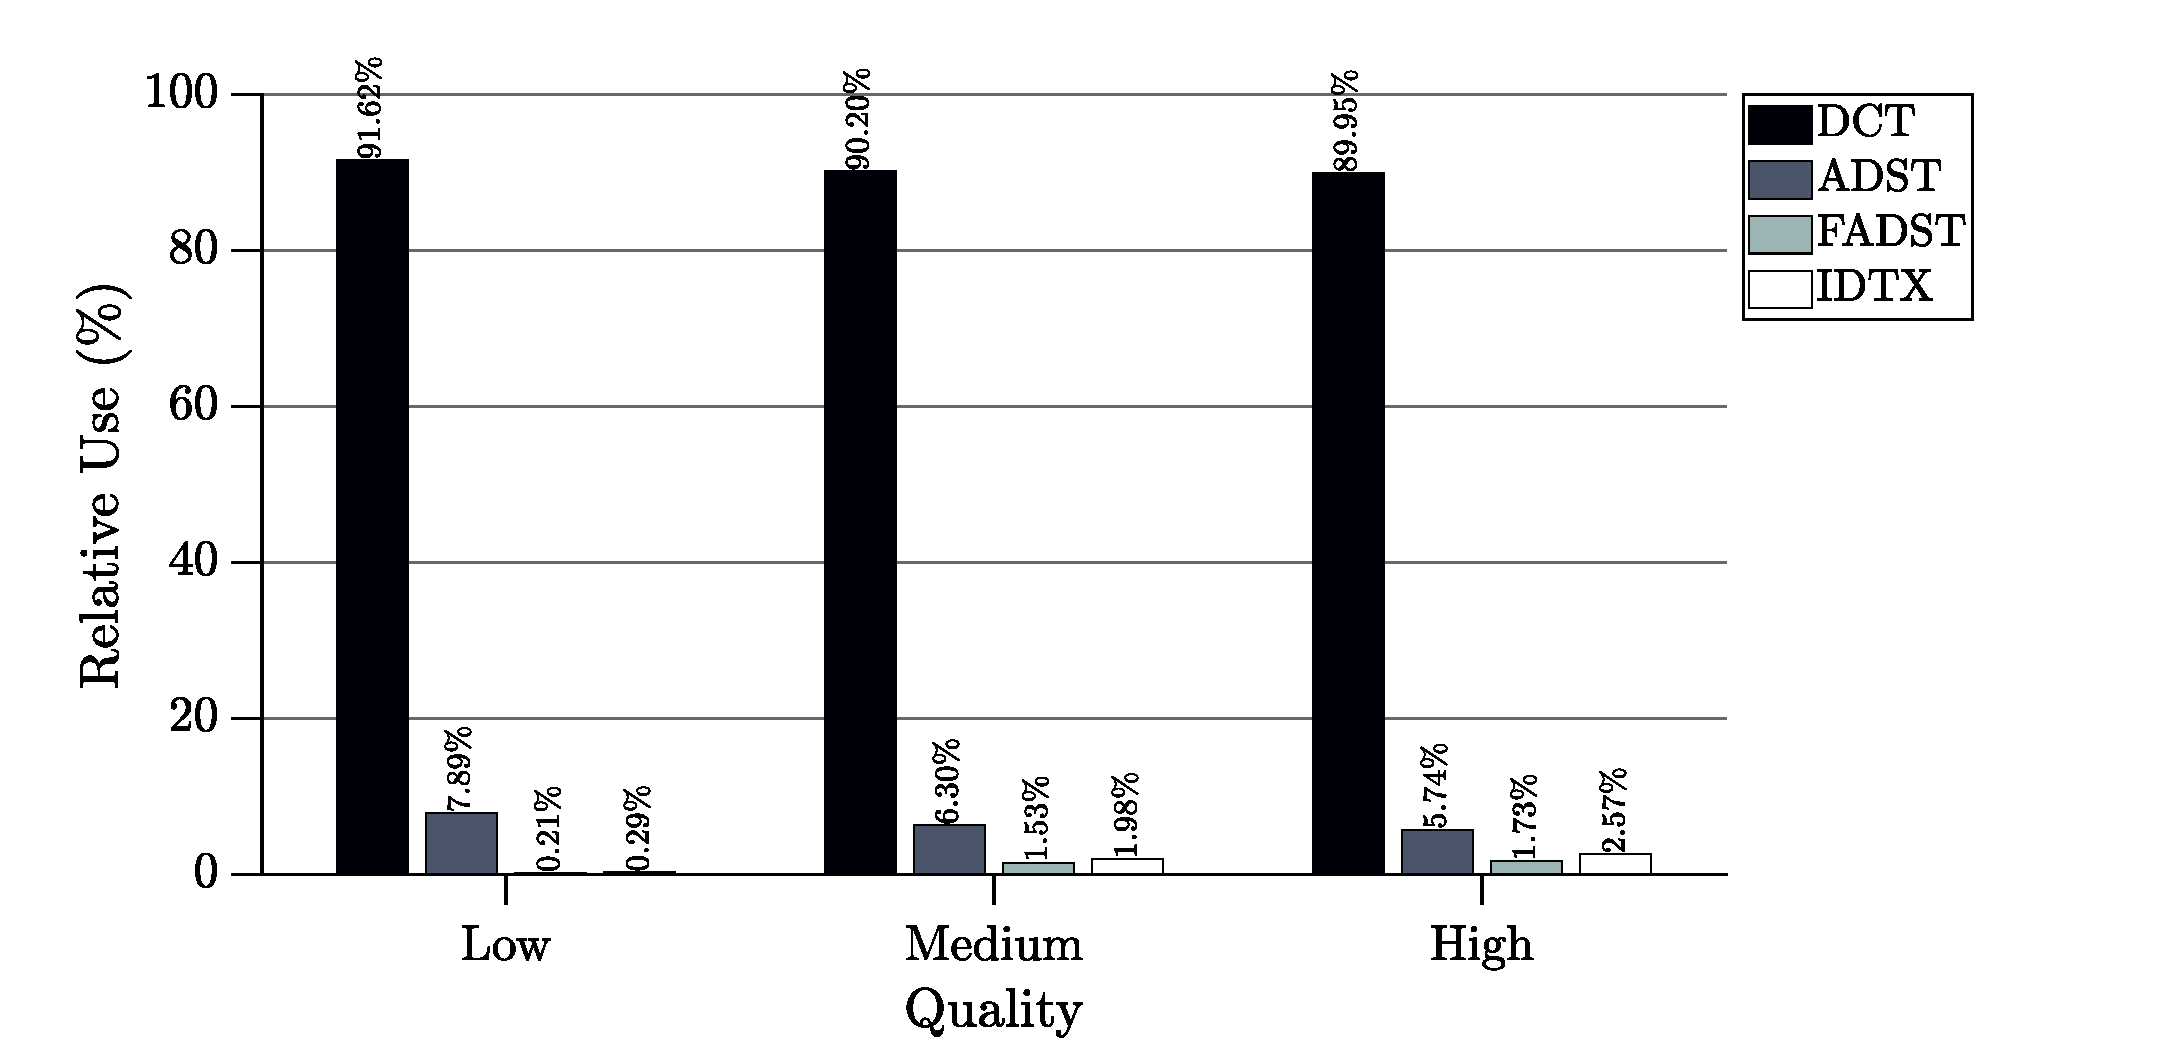
\includegraphics[width=\textwidth]{Figures/kernelAvg.eps}
                            \caption{Kernel Utilizado}
                     \end{figure}
       \end{center}
\end{frame}

\note{
       \begin{itemize}[label=$\bullet$]
              \item DCT é a mais utilizada
              \item Outros kernels só são utilizados em objetivos de qualidade mais elevados
       \end{itemize}
}

\begin{frame}
       \frametitle{Opções de Codificação - Resultados}              
       \begin{center}
                     \begin{figure}[h]
                            \centering
                            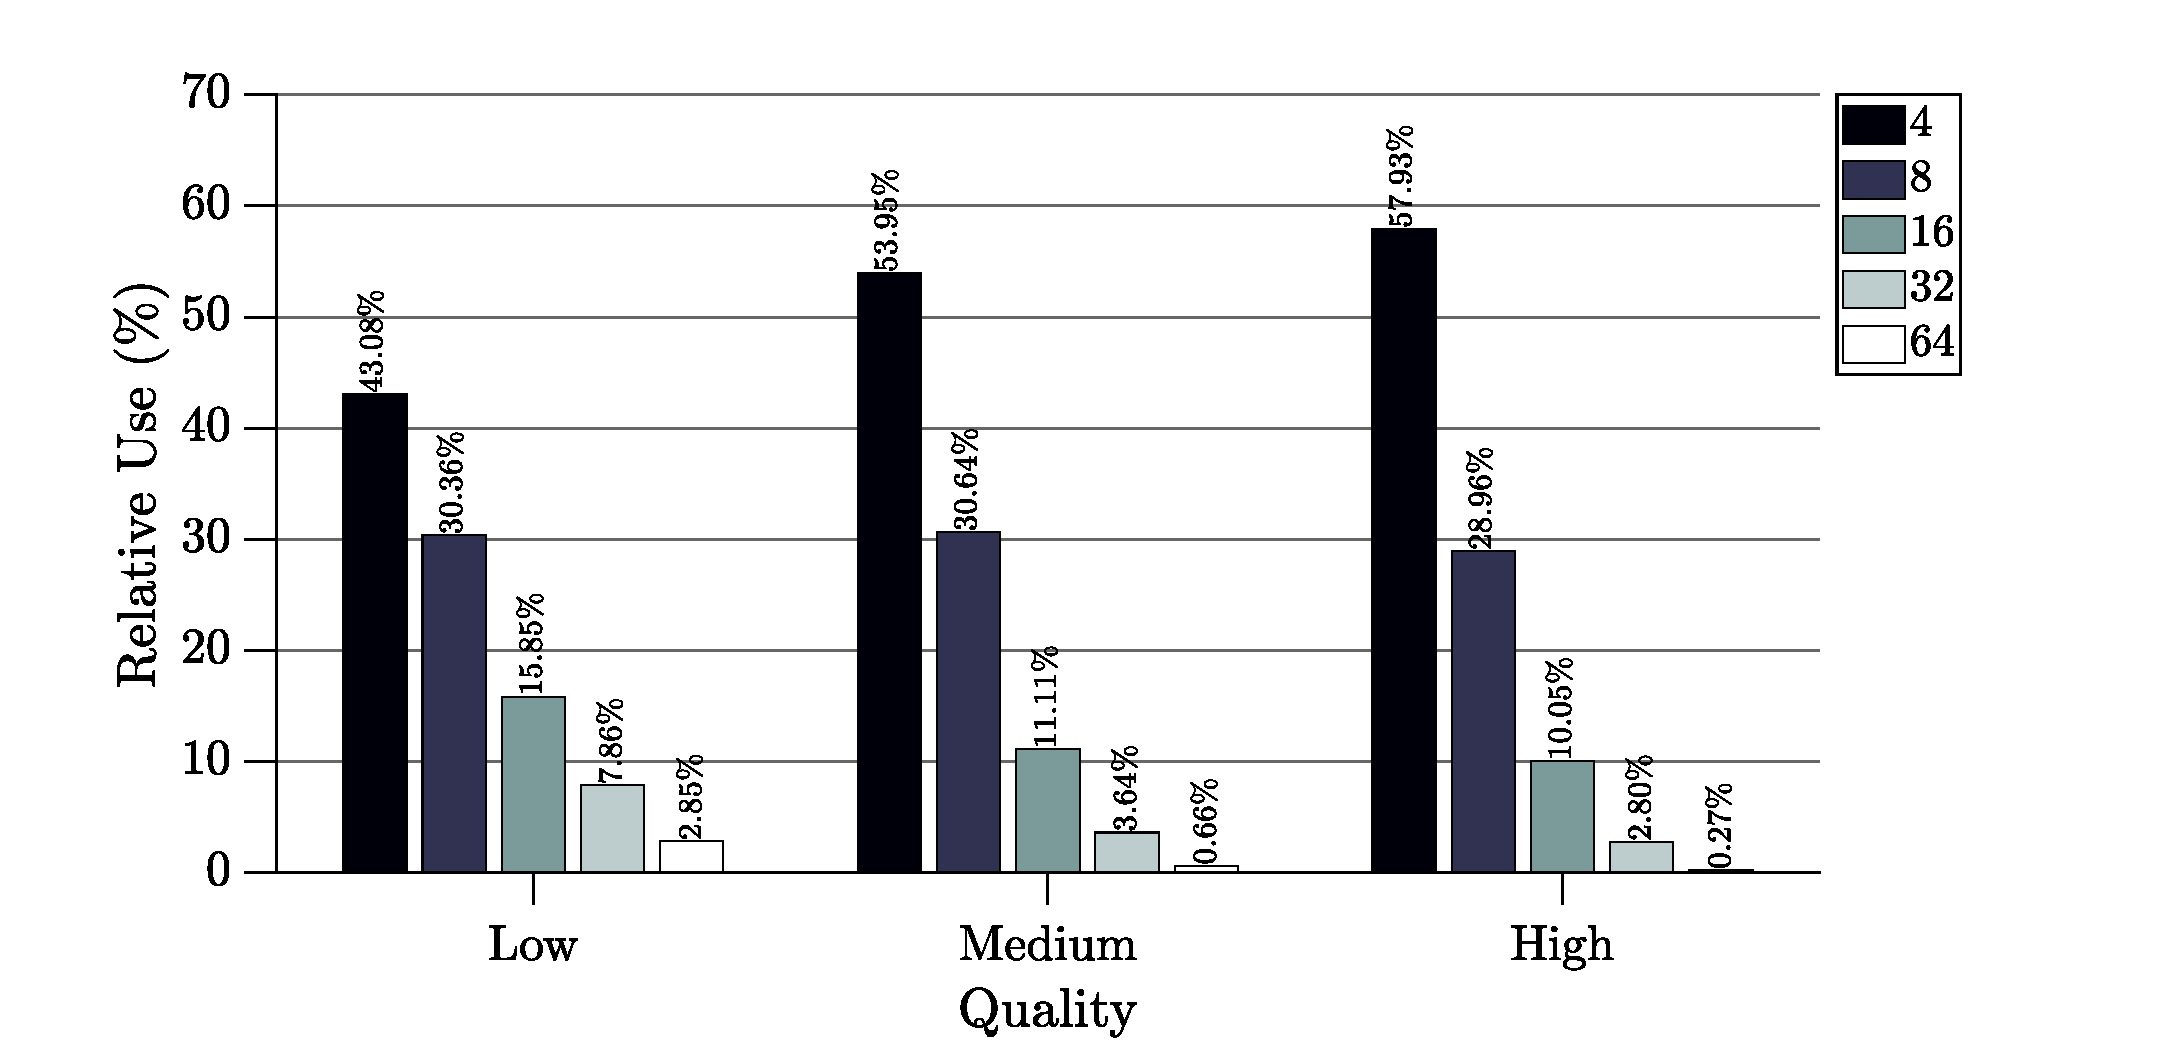
\includegraphics[width=\textwidth]{Figures/vectSizAvg.eps}
                            \caption{Tamanho de Vetor}
                     \end{figure}
       \end{center}
\end{frame}

\note{
       \begin{itemize}[label=$\bullet$]
              \item A dimensão mais comum é 4, e o seu uso aumenta com a qualidade pretendida
              \item Esperado, pois para uma dada area de imahem ser transformada com vetores de 1 por 4, tem que ser feitas mais trnaformaçoes do que para vetores de dimensoes superiores
       \end{itemize}
}

\begin{frame}
       \frametitle{Opções de Codificação - Resultados}              
       \begin{center}
                     \begin{figure}[h]
                            \centering
                            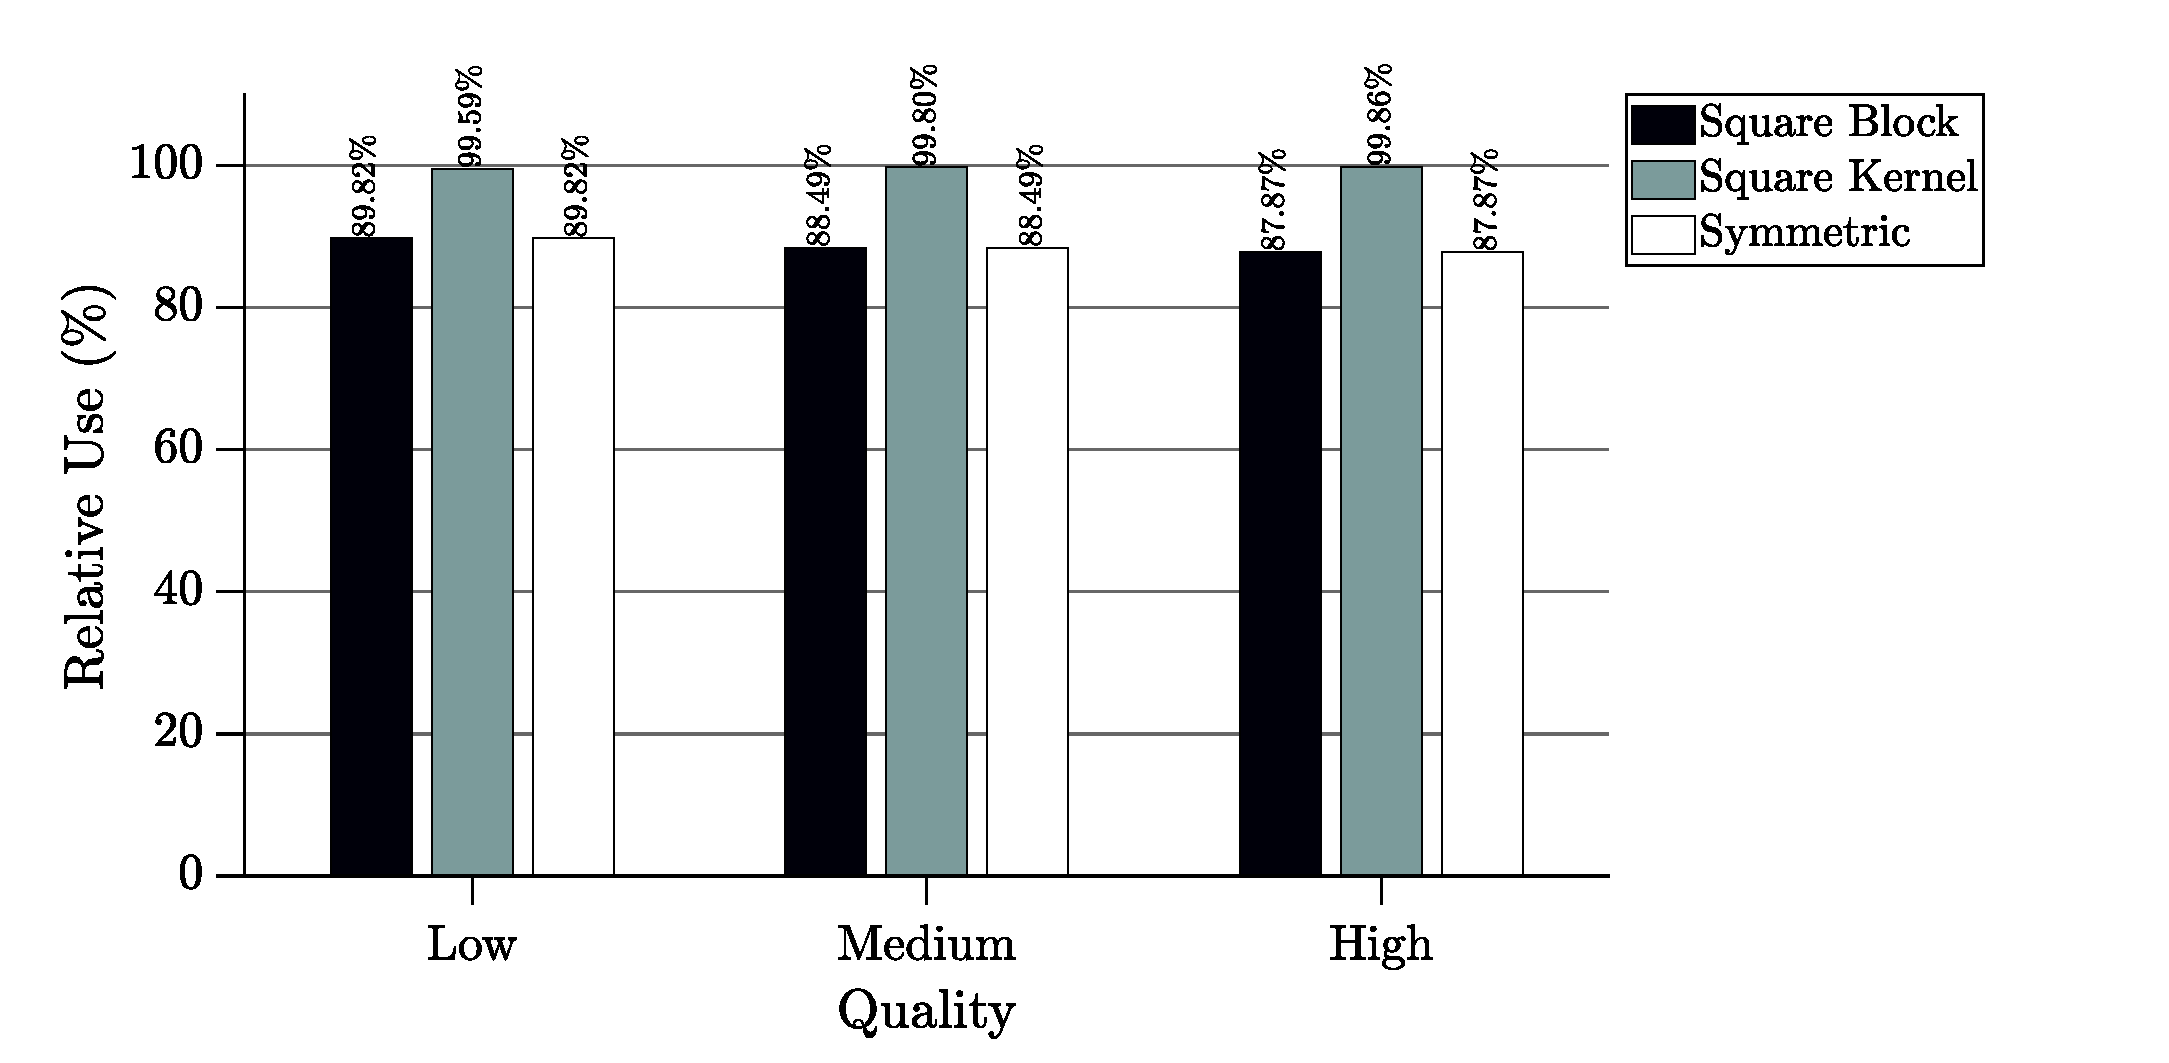
\includegraphics[width=\textwidth]{Figures/squareAvg.eps}
                            \caption{Kernel Simétrico}
                     \end{figure}
       \end{center}
\end{frame}

\note{
       \begin{itemize}[label=$\bullet$]
              \item É possível verificar a percentagem de ocurrencias para kernels simétricos (tamanho e kernel de colunas igual a tamanho e kernel de linhas)
       \end{itemize}
}

\begin{frame}
       \frametitle{Opções de Codificação - Resultados}              
       \begin{center}
                     \begin{figure}[h]
                            \centering
                            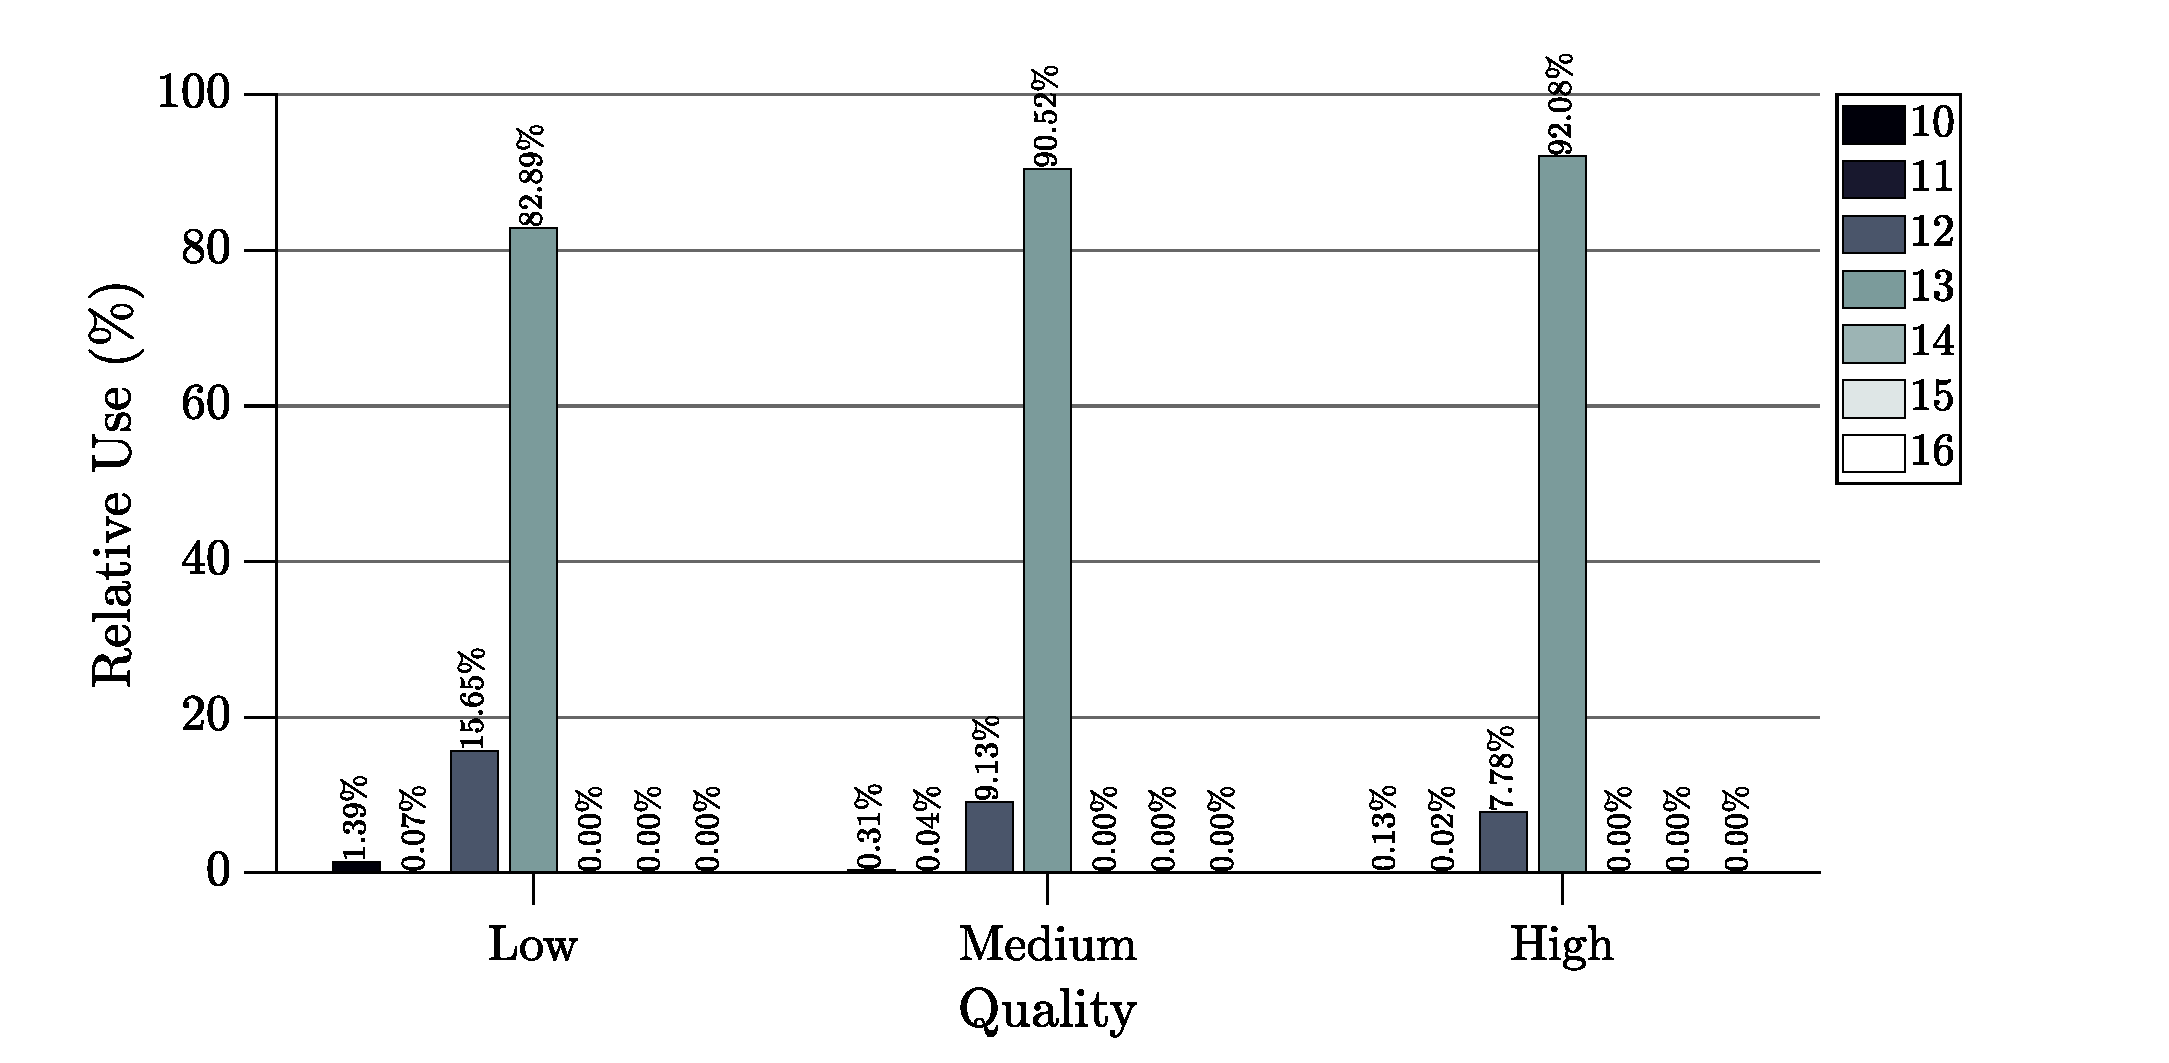
\includegraphics[width=\textwidth]{Figures/cosBitAvg.eps}
                            \caption{Número de Bits Utilizados nas Aproximações do Cosseno}
                     \end{figure}
       \end{center}
\end{frame}

\note{
       \begin{itemize}[label=$\bullet$]                                   
              \item A maior parte das transformações usa 13 bits para as representações dos cossenos
              \item À medida que a qualidade aumenta, também aumenta o numero de bits no cosseno       
       \end{itemize}
}       

\begin{frame}
       \frametitle{Nº de bits dos Cossenos vs Distorção - Teste}
       \begin{figure}[h]
              \centering
              \begin{tikzpicture}[%
    >=triangle 60,              % Nice arrows; your taste may be different
    start chain=going right,    % General flow is top-to-bottom
    node distance=2cm,          % Global setup of box spacing
    every join/.style={norm},   % Default linetype for connecting boxes
    ]

\tikzset{
    base/.style={draw, on chain, on grid, align=center},
    proc/.style={base, rectangle, text width=2cm, fill=black!10, minimum height=1.5cm, minimum width=1.5cm,font={\bfseries}},    
    frame/.style={base, minimum height=1.5cm, minimum width=2cm, fill=blue!10, thick},
    sub/.style={base, circle, inner sep=0pt, radius=0.4cm, fill=black!10, minimum height=3.5ex, font={\bfseries}},
    spot/.style={circle, inner sep=0pt, radius=0.4cm, minimum height=2mm, draw},
    edge rectangle/.style={ to path={ rectangle (\tikztotarget)}},
    % coord node style is used for placing corners of connecting lines
    coord/.style={coordinate, on chain, on grid, node distance=6mm and 40mm},
    % Arrows 
    fforw/.style={->, thick},
    fback/.style={->, thick, red!75!black},
    aref/.style={<->, dashed, black!50},
    % -------------------------------------------------
    % Connector line styles for different parts of the diagram
    cascaded/.style = {%
    general shadow = {%
      shadow scale = 1,
      shadow xshift = -1ex,
      shadow yshift = 1ex,
      draw,
      thick,
      fill = blue!40},
    general shadow = {%
      shadow scale = 1,
      shadow xshift = -.5ex,
      shadow yshift = .5ex,
      draw,
      thick,
      fill =blue!40},
    fill = blue!40, 
    draw,
    thick,
    minimum width = 2cm,
    minimum height = 1.5cm,
    font={\itshape}},
    base
}

%% Reference
\node [cascaded] (inseq) {Input\\Sequence\\$g$};

\node [proc, right=3cm of inseq] (regenc) {Regular\\Encoder};
    \draw[->] (inseq) -- (regenc);
\node [proc, above=of regenc] (bit10enc) {10 bit\\Encoder};
    \draw[->] (inseq)+(1.5cm,0) |- (bit10enc);
\node [proc, below=of regenc] (bit16enc) {16 bit\\Encoder};
    \draw[->] (inseq)+(1.5cm,0) |- (bit16enc);

\node [proc, right=3cm of regenc] (dec) {Decoder};
    \draw[->] (regenc) -- (dec);
    \draw[->] (bit10enc) --++(1.5cm,0) |- (dec.160);
    \draw[->] (bit16enc) --++(1.5cm,0) |- (dec.200);

\node [cascaded, right=3.5cm of dec] (regrec) {Regular\\Reconstructed};
    \draw[->] (dec) -- ([xshift=-1.3mm]regrec.west);
\node [cascaded, above=of regrec] (10bitrec) {10 bit\\Reconstructed};
    \draw[->] (dec.20) --++(0.5cm,0) |- ([xshift=-1.3mm]10bitrec.west);
\node [cascaded, below=of regrec] (16bitrec) {16 bit\\Reconstructed};
    \draw[->] (dec.340) --++(0.5cm,0) |- ([xshift=-1.3mm]16bitrec.west);

\node [proc, right=3cm of regrec, fill=black!15] (psnr) {Calculate \emph{PSNR}};
    \draw[->] (regrec) -- (psnr);
    \draw[->] (10bitrec) --++(1.5cm,0) |- (psnr.160);
    \draw[->] (16bitrec) --++(1.5cm,0) |- (psnr.200);

    \node[coord, below=3cm of inseq] (a) {};
    \node[coord, below=3cm of psnr] (aa) {};
    \draw[->] (inseq) -- (a) -- (aa) -- (psnr);
\end{tikzpicture}  
              \caption{Testes de codificação com diferentes bits nas aproximações de cosseno}            
       \end{figure}
\end{frame}

\note{
       \begin{itemize}[label=$\bullet$]
              \item Poderá levar a pensar que o número de bits do cosseno influencia a qualidade da imagem
              \item Testes feitos para avaliar esta hipotese
              \item Testes de codificação forçando o número de bits utilizados nas aproximações dos cossenos, no codificador
              \item Descodificação feita com o descodificador de origem, que usa sempre 12 bits
              \item Cálculo da Relação Sinal Ruído de Pico e comparar com os tres codificadores, para os tres objetivos de qualidade distintos
       \end{itemize}
}

\begin{frame}
       \frametitle{Nº de bits dos Cossenos vs Distorção - Resultados}
       \begin{figure}[h]
              \centering
              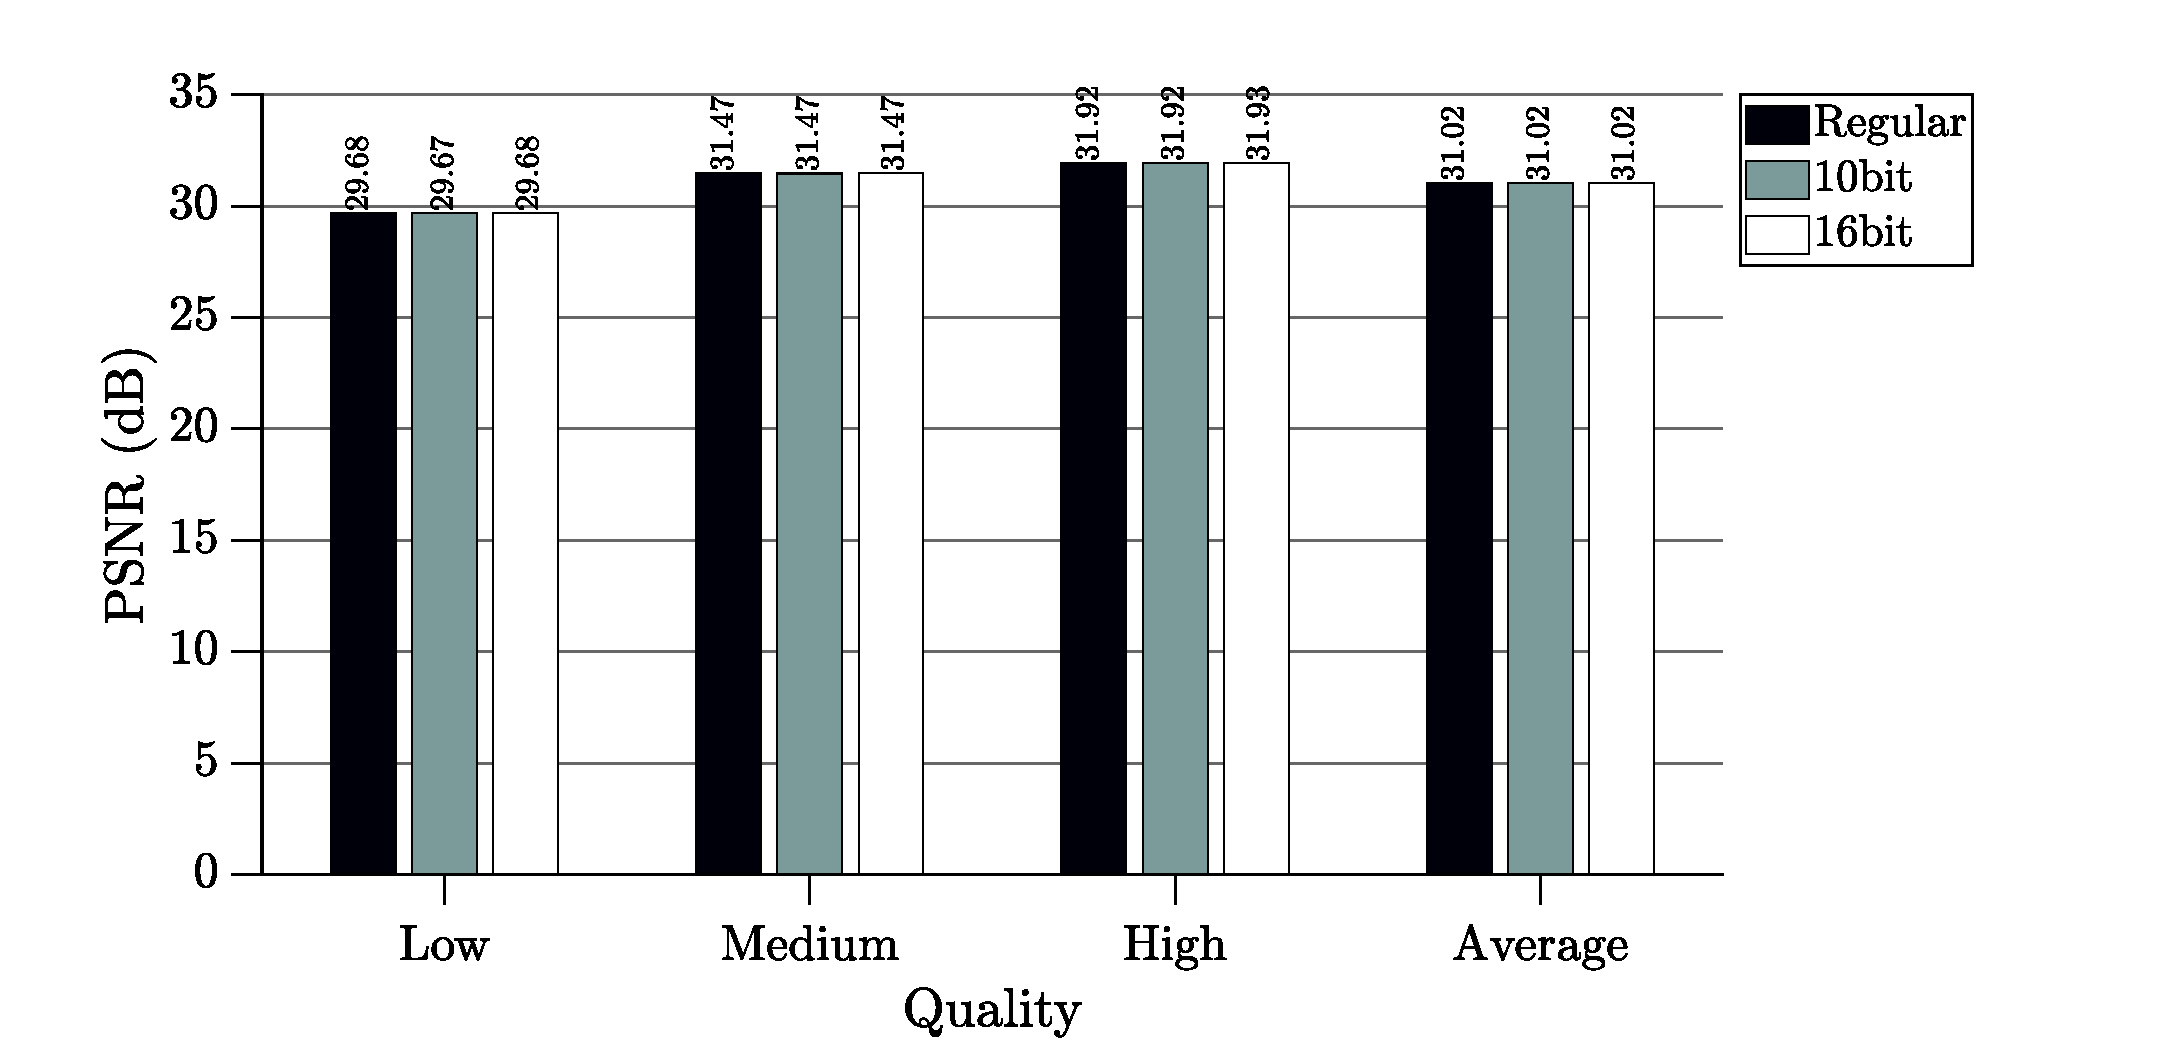
\includegraphics[width=\textwidth]{Figures/compcosbitAvg.eps}
              \caption{Comparaçao Distorção com Número de Bits usados no Cosseno}
       \end{figure}
\end{frame}

\note{
       \begin{itemize}[label=$\bullet$]
              \item PSNR independente do número de bits utilizado no cosseno, para qualquer objetivo de qualidade
              \item Princípio de base para otimização do software de referencia
              \item Outros aspetos podem ser explorados para a otimização do software de referencia
       \end{itemize}
}

%%%%%%%%%%%%%%%%%%%%%%
% Arquiteturas Desenvolvidas
\metroset{sectionpage=none}
\section{Arquiteturas Propostas}

\subsection{Software}

\note{
       \begin{itemize}[label=$\bullet$]
              \item Foco na DCT pois seria a que causaria mais impacto na performance do encoder
       \end{itemize}
}

\begin{frame}
       \frametitle{Redução do Número de Bits}
       \begin{figure}[h]
              \centering
              \begin{tikzpicture}[%
    >={Triangle[length=6pt,angle'=28]},
    start chain=going below,    % General flow is left-to-right
    node distance=2mm and 20mm, % Global setup of box spacing
    every join/.style={norm},   % Default linetype for connecting boxes
    scale=0.8, every node/.style={transform shape},
    ]
\tikzset{
  base/.style={draw, on chain, on grid, align=center, minimum height=3.5ex},
  inout/.style={base,trapezium,trapezium left angle=70,trapezium right angle=-70, fill=black!12},
  sum/.style={base, circle, inner sep=0pt, radius=0.4cm, fill=black!8},
  ar/.style={->, line width=0.4mm},
  nar/.style={ar, red!75!black},
  pathcos/.style={font=\small, sloped}
}
    \node [inout] (a3) {$A$};
    \node [inout] (b3) {$B$};
    \path (a3) -- (b3) node [midway] (s3t) {};
    \node [sum, right=of s3t] (s3) {\textbf{+}};
        \path (a3.east) to node [pathcos, above, near start] {$\alpha$} (s3.west);
            \draw [ar] (a3.east) -- (s3);
        \path (b3.east) to node [pathcos, color=red!75!black, below, near start] {$\beta$} (s3.west);
            \draw [nar] (b3.east) -- (s3);
    \node [inout, right=of s3] (c3) {$C$};
        \draw [ar] (s3) -- (c3);
    \node [right=1cm of c3] (eq3) {C = ($\alpha\cdot$A + $\beta\cdot$B)\texttt{>>}8};
\end{tikzpicture}
              \caption{Operação implementada nas transformadas inteiras}
       \end{figure}
       \begin{columns}
              \column{0.5\textwidth}
                     \begin{equation*}
                            M_{original} = 728\, B
                     \end{equation*}
                     \begin{equation*}
                            M_{8 bits} = 64\, B \approx 0.2\cdot M_{original}
                     \end{equation*}
              \column{0.5\textwidth}
                     \begin{gather*}
                            \Delta_{10} = \frac{1-0}{2^{10}} \approx 0.98\cdot10^{-3}\\
                            \Delta_{8} = \frac{1-0}{2^{8}} \approx 3.9\cdot10^{-3}\\
                            \Downarrow \\
                            MSE_{8} = 16\cdot MSE_{10} 
                     \end{gather*}
       \end{columns}
\end{frame}

\note{
       \begin{itemize}[label=$\bullet$]
              \item Testar a hipótese da redução de complexidade pela redução do número de bits dos cossenos
              \begin{itemize}[label=$\bullet$]
                     \item Multiplicações mais simples
                     \item Número de Shifts reduzido
              \end{itemize}
              \item Teste com 8 bits
              \item levaria à redução em 81\% da memória utilizada para armazenamento destas aproximações
              \item Possibilidade de degradação da qualidade de imagem pois o Erro de Quantização Quadrático médio aumentaria em 16 vezes
              \item Repetição dos testes de distorção usando encoder com 8 bits e encoder original
       \end{itemize}
}

\begin{frame}
       \frametitle{Otimização do \emph{libaom}}       
       \begin{center}
                     \begin{figure}[h]
                            \centering
                            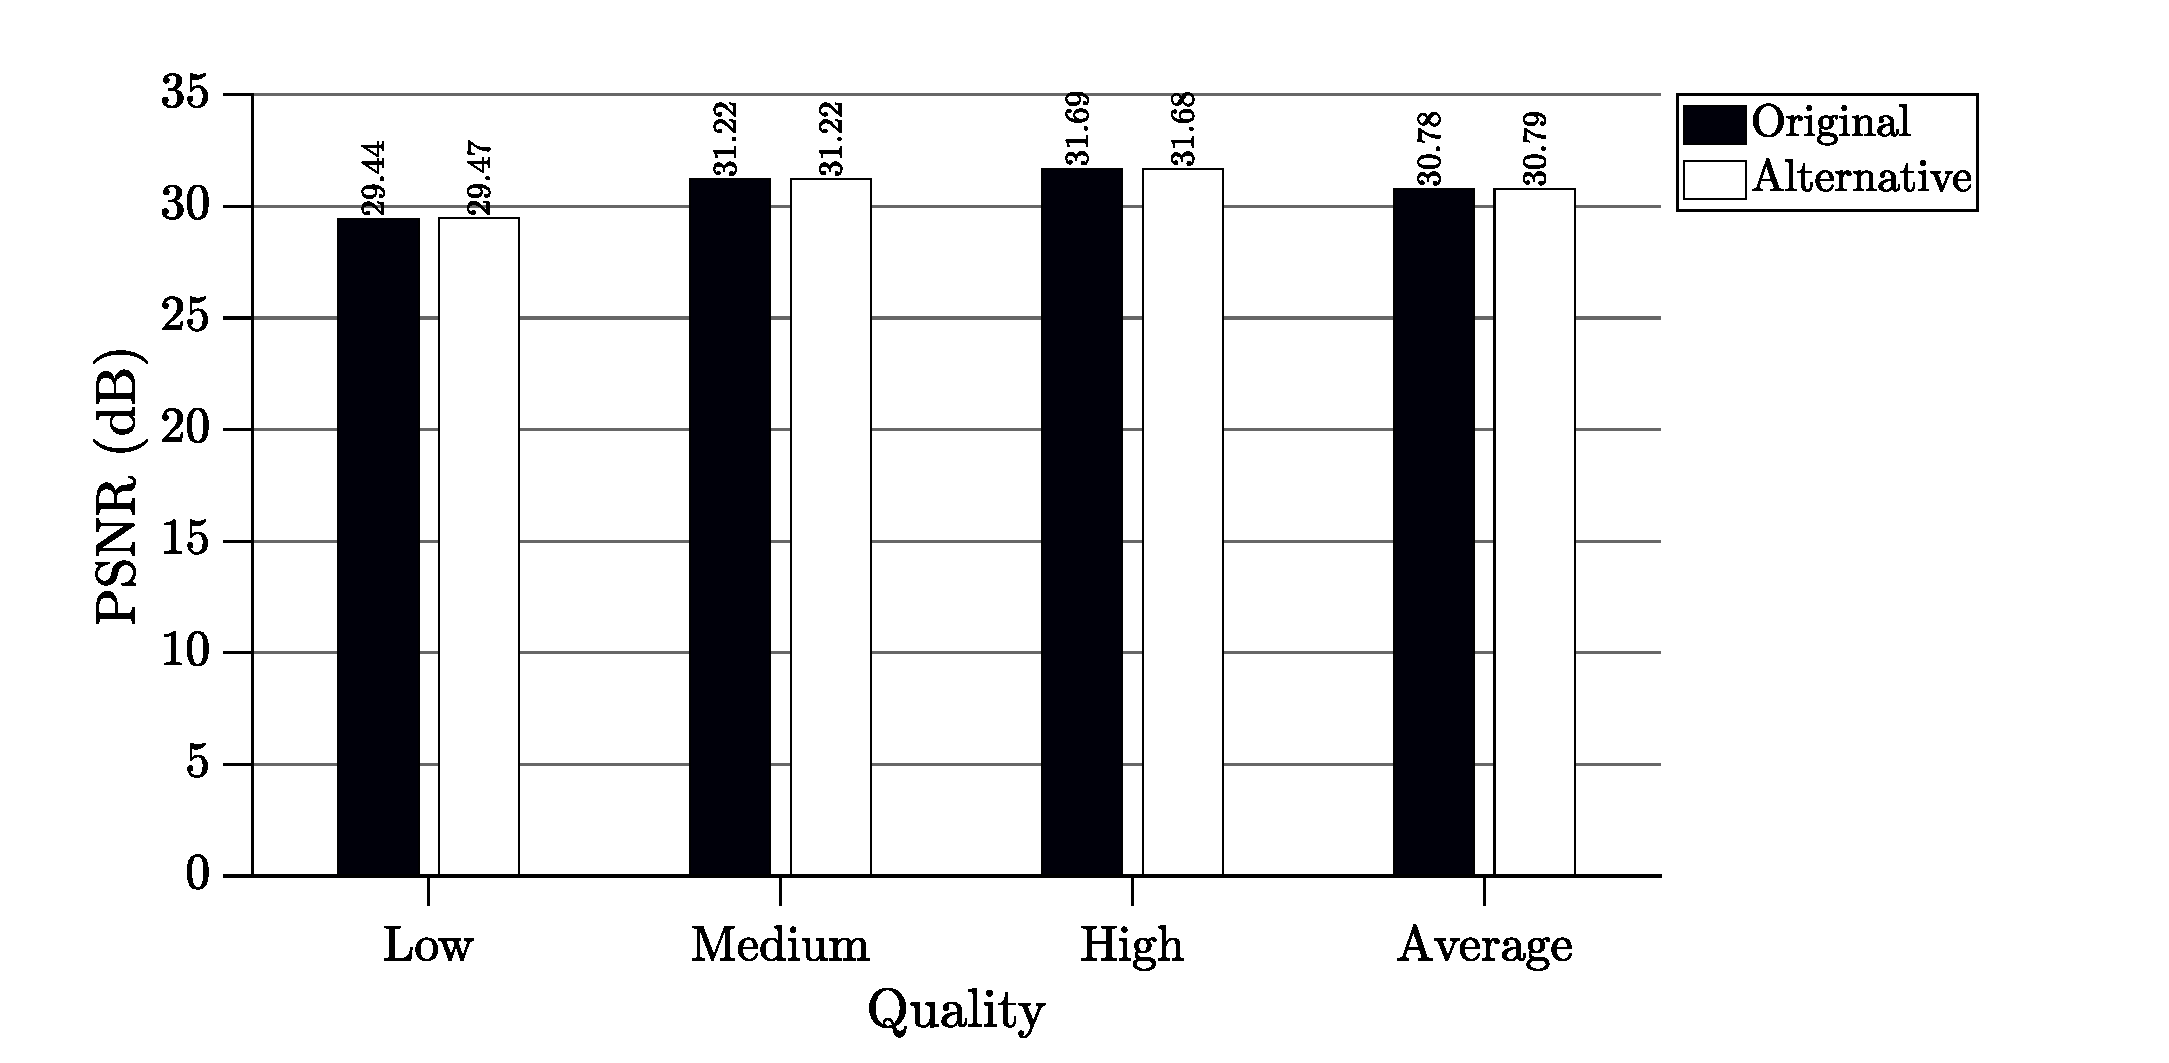
\includegraphics[width=\textwidth]{Figures/buttmultqual.eps}
                            \caption{Comparação da distorção}
                     \end{figure}
       \end{center}
\end{frame}

\note{
       \begin{itemize}[label=$\bullet$]
              \item É possível verificar a percentagem de ocurrencias para kernels simétricos (tamanho e kernel de colunas igual a tamanho e kernel de linhas)
       \end{itemize}
}

\begin{frame}
       \frametitle{Otimização do \emph{libaom}}       
       \begin{center}
                     \begin{figure}[h]
                            \centering
                            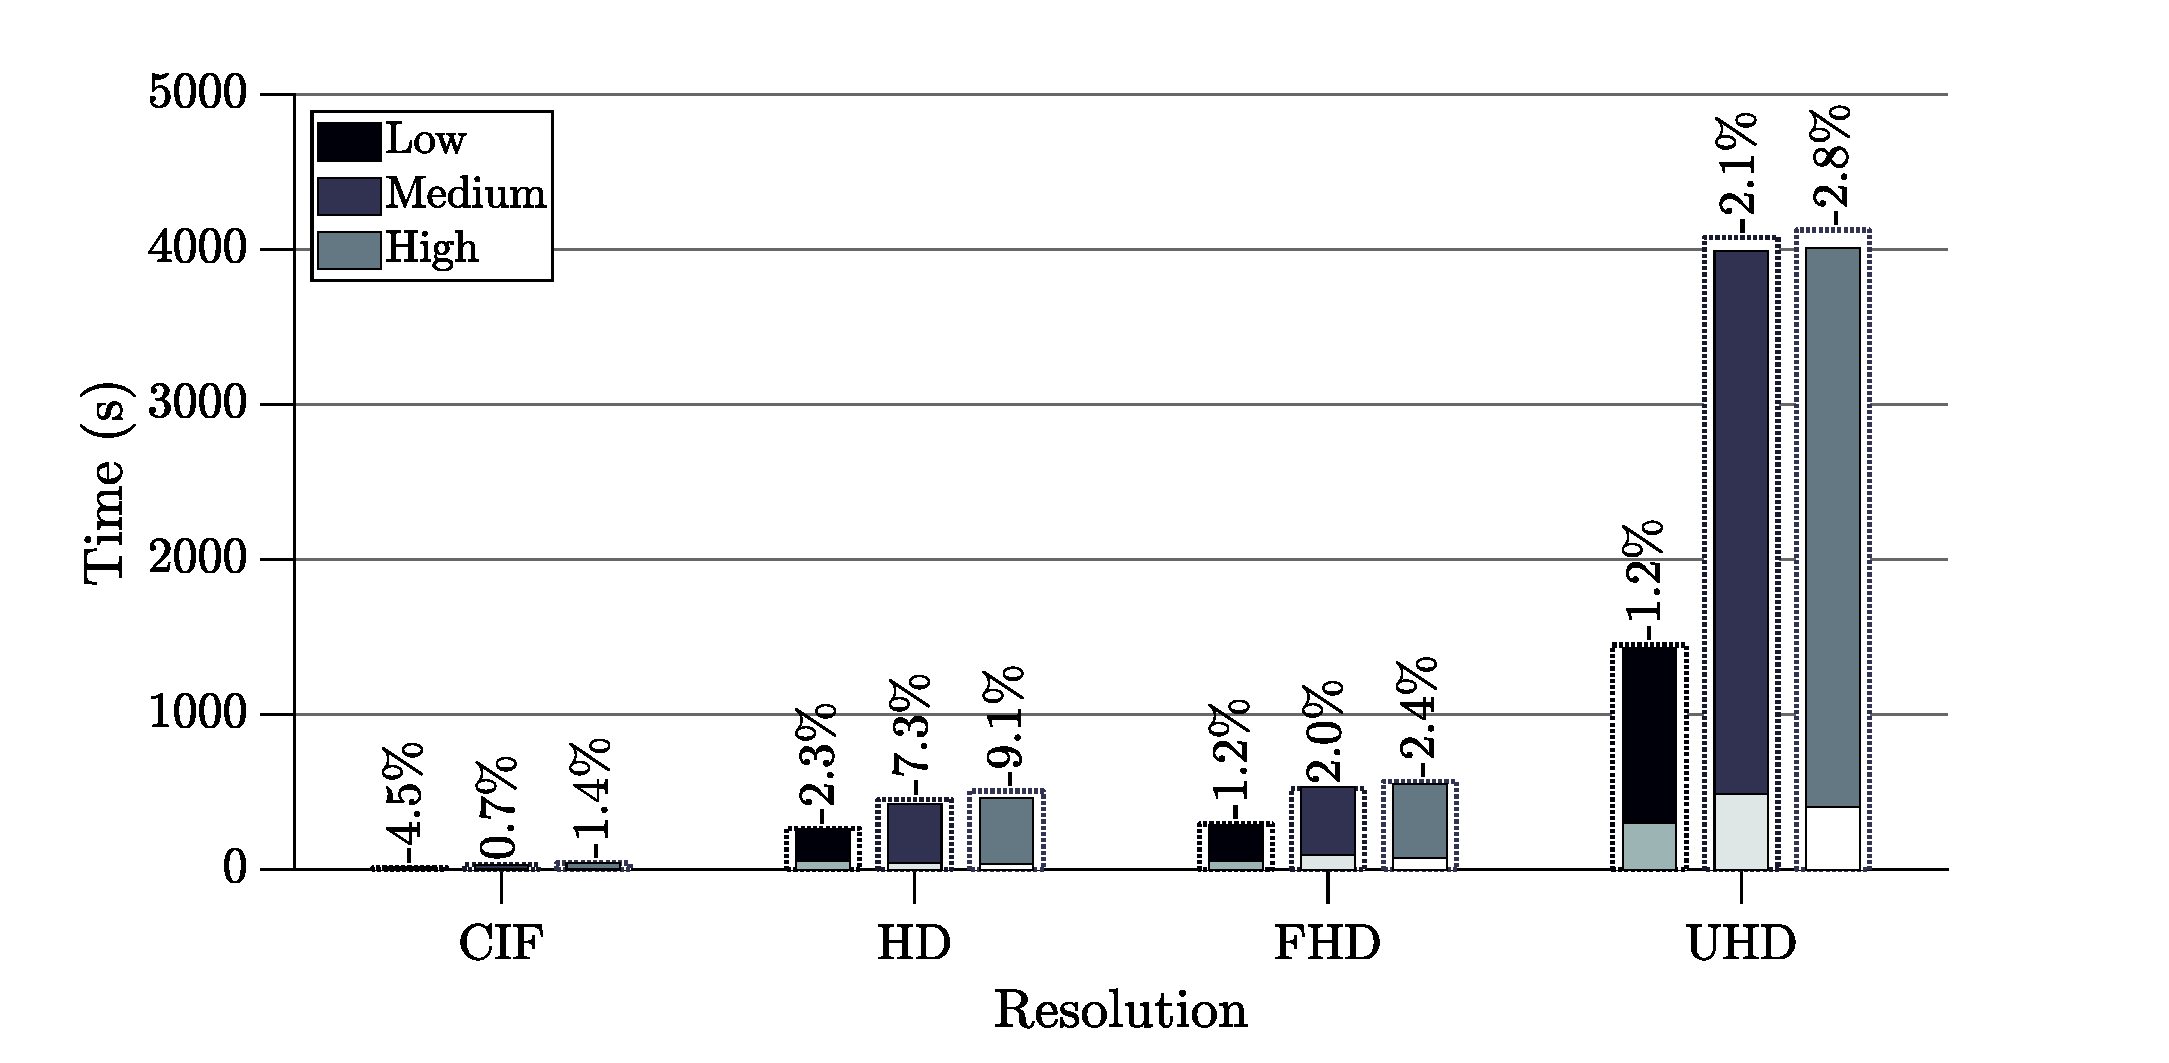
\includegraphics[width=\textwidth]{Figures/buttmulttime.eps}
                            \caption{Tempo de Codificação}
                     \end{figure}
       \end{center}
\end{frame}

\note{
       \begin{itemize}[label=$\bullet$]              
              \item Redução de 3\% no tempo de codificação:
              \begin{itemize}[label=$\bullet$]
                     \item Tracejado: Tempo de codificação com codificador original
                     \item Barras escuras: Tempo de codificação do codificador modificado
                     \item Barras claras: tempo da Transformada
                     \item Percentagem: Diferença percetual do tempo entre codificador original e codificador modificado
              \end{itemize}              
       \end{itemize}
}

\subsection{Hardware}

\note{
       \begin{itemize}[label=$\bullet$]
              \item Com o estudo do software de referencia feito
              \item Avanço para arquiteturas em hardware
       \end{itemize}
}

\metroset{sectionpage=progressbar}
\begin{frame}
       \frametitle{Princípios de desenvolvimento}
       \begin{figure}[h]
              \centering
              \input{Figures/av1_fdct8_deconstruct.tex}
              \caption{Estágios da DCT inteira}
       \end{figure}
\end{frame}

\note{
       \begin{itemize}[label=$\bullet$]
              \item Desenvolvimento foi feito em VHDL no Vivado da Xilinx
              \item Designs e sinteses feitas com objetivo de implementação em Artix 7
              \item Cada estágio é feito sequencialmente
              \item Estágios de somas simples e de Multiplicação, Soma e Shift
       \end{itemize}
}

\begin{frame}
       \frametitle{Princípios de desenvolvimento}
       \begin{figure}[h]
              \centering
              \begin{tikzpicture}[%
    >={Triangle[length=6pt,angle'=28]},
    start chain=going below,    % General flow is left-to-right
    node distance=5mm and 16mm, % Global setup of box spacing
    every join/.style={norm},   % Default linetype for connecting boxes
    scale=0.7, every node/.style={transform shape},
    ]

    \tikzset{
    base/.style={draw, on chain, on grid, align=center, minimum height=3.5ex},
    proc/.style={base, rectangle, fill=black!10},
    inout/.style={base,trapezium,trapezium left angle=70,trapezium right angle=-70, fill=black!12},
    term/.style={proc, rounded corners},
    sum/.style={base, circle, inner sep=0pt, radius=0.4cm, fill=black!8},
    % coord node style is used for placing corners of connecting lines
    coord/.style={coordinate, on chain, on grid, node distance=6mm and 40mm},
    % nmark node style is used for coordinate debugging marks% -------------------------------------------------
    % Connector line styles for different parts of the diagram
    norm/.style={ar, draw},
    free/.style={ar, draw, green3},
    cong/.style={ar, draw, red3},
    it/.style={font={\small\itshape}},
    ar/.style={->, line width=0.4mm},
    nar/.style={ar, red!75!black},
    pathcos/.style={font=\small, sloped}
    }

    \begin{scope}        
        \node [inout] (x1) {\texttt{x1}};
        \node [sum, right=of x1, join] (s1) {$\mathbf{\times}$};
        \node [proc, above=1cm of s1] (a) {\texttt{a}};
            \draw[ar] (a) -- (s1);

        \node [inout, below=1cm of x1] (x2) {\texttt{x2}};      
        \node [sum, right=of x2, join] (s2) {$\mathbf{\times}$};
        \node [below=1cm of s2, proc] (b) {\texttt{b}};
            \draw[ar] (b) -- (s2);

        \node [below left=3.5cm and 1cm of x2, align=center, font={\bfseries}] (clk) {Sinal de\\Relógio};
            \draw[thick] ($(clk.east)+(0.5,0)$) -- (x2 |- clk.east) -- ++(0,0.5) coordinate (inReg) -- ++(0.8,0) -- ++(0,-0.5) -- ++(0.8,0) -- ++(0,0.5) coordinate (mult) -- ++(0.8,0) -- ++(0,-0.5) -- ++(0.8,0) -- ++(0,0.5) coordinate (sum) -- ++(0.8,0) -- ++(0,-0.5) -- ++(0.8,0) -- ++(0,0.5) coordinate (shift) -- ++(0.8,0) -- ++(0,-0.5) -- ++(0.8,0) -- ++(0,0.5) coordinate (out) -- ++(0.8,0);
        
        \node[align=center,anchor=north, font={\bfseries\small}, yshift=21mm, draw=darkgray, thin] (lab1) at (mult) {Multiplicação};
            \draw[dashed] (mult) --(lab1);
        \node[align=center,anchor=north, font={\bfseries\small}, yshift=12mm, draw=darkgray, thin] (lab2) at (sum) {Soma};
            \draw[dashed] (sum) --(lab2);
        \node[align=center,anchor=north, font={\bfseries\small}, yshift=7mm, draw=darkgray, thin] (lab3) at (shift) {Shift};
            \draw[dashed] (shift) --(lab3);

        \path (s1) -- (s2) node[midway, rotate=90] (mid_s) {};
        \node [sum, right=of mid_s] (s3) {$\mathbf{+}$};
            \draw[ar] (s1.east) -- (s3);
            \draw[ar] (s2.east) -- (s3);

        \node[draw, fill=black!10, right=16mm of s3.center, anchor=center] (sh8) {\texttt{>>8}};
            \draw[ar] (s3) -- (sh8);

        \node[inout, right=of sh8, anchor=center] (y) {\texttt{y}};
            \draw[ar] (sh8) -- (y);

        \path (x1) -- (x2) node[midway, rotate=90] (mid_x) {};
        \path (mid_x) -- (y) node[midway, rotate=90] (center) {};        
        \node[above=3cm of center] (eq) {\texttt{y = (a*x1 + b*x2)>>8;}};        
    \end{scope}

    \begin{pgfonlayer}{background}
        \path (clk.west |- a.north)+(-5mm,2mm) node (a11) {};
        \path (y.east |- clk.south)+(20mm,-2mm) node (a21) {};
        \path[fill=black!2,rounded corners, draw=black!50, dashed]
          (a11) rectangle (a21);
        \path (y.east |- a.north)+(20mm,2mm) node (a22) {};
            \path (a21) -- (a22) node[midway, rotate=90, yshift=0.5cm] (mid_right) {\textbf{Hardware}};

        \path (clk.west |- eq.north)+(-5mm,7mm) node (a11) {};
        \path (y.east |- eq.south)+(20mm,-7mm) node (a21) {};
        \path[fill=black!2,rounded corners, draw=black!50, dashed]
          (a11) rectangle (a21);
        \path (y.east |- eq.north)+(20mm,7mm) node (a22) {};
            \path (a21) -- (a22) node[midway, rotate=90, yshift=0.5cm] (mid_right) {\textbf{Software}};
    \end{pgfonlayer}
\end{tikzpicture}
              \caption{Implementação de operação de software em hardware}
       \end{figure}
\end{frame}

\note{
       \begin{itemize}[label=$\bullet$]
              \item em software é uma operação fácil, descrita numa linha de códigos
              \item em hardware tem que ser decomposta em três estágios diferentes
              \item controlado pelo flanco ascendente de um sinal de clock
       \end{itemize}
}

\begin{frame}
       \frametitle{Princípios de desenvolvimento}
       \begin{figure}[h]
              \centering
              \input{Figures/av1_fdct8_deconstruct2.tex}
              \caption{Inclusão de DCT4 na DCT8}
       \end{figure}
\end{frame}

\note{
       \begin{itemize}[label=$\bullet$]
              \item Operações das DCTs mais pequenas são contidas nas DCTs de maiores dimensões
              \item Comportamento replica-se para os restantes tamanhos
              \item Permite repetição de hardware, simplificando o desenvolvimento
       \end{itemize}
}

\begin{frame}[c]
       \begin{figure}[h]
              \centering
              \begin{minipage}{.75\textwidth}
                     \begin{tikzpicture}[%
    >={Triangle[length=6pt,angle'=28]},
    start chain=going below,    % General flow is left-to-right
    node distance=5mm and 20mm, % Global setup of box spacing
    every join/.style={norm},   % Default linetype for connecting boxes
    ]

\tikzset{
  base/.style={draw, on chain, on grid, align=center, minimum height=3.5ex},
  reg/.style={base, rectangle, minimum width=2.5em, minimum height=2em,fill=black!15},
  proc/.style={base, rectangle, minimum width=4em, minimum height=8em, fill=black!15},
  inout/.style={base,trapezium,trapezium left angle=70,trapezium right angle=-70, fill=blue!12},
  term/.style={proc, rounded corners},
  sum/.style={base, circle, inner sep=0pt, radius=0.4cm, fill=black!15},
  % coord node style is used for placing corners of connecting lines
  coord/.style={coordinate, on chain, on grid, node distance=6mm and 40mm},
  % nmark node style is used for coordinate debugging marks% -------------------------------------------------
  % Connector line styles for different parts of the diagram
  norm/.style={aar, draw},
  free/.style={aar, draw, green3},
  cong/.style={aar, draw, red3},
  it/.style={font={\small\itshape}},
  nar/.style={aar, red!75!black},
  aar/.style={->, line width=0.4mm},
  pathcos/.style={font=\small, sloped}
}    

\begin{scope}


\end{scope}
\end{tikzpicture}
                 \end{minipage}  
                 \hspace{-1cm}
                 \begin{minipage}[]{.25\textwidth}
                     \caption{Implementação em hardware da DCT4}
                 \end{minipage}
       \end{figure}
\end{frame}

\note{
       \begin{itemize}[label=$\bullet$]
              \item Arquitetura mais simples
              \item Ativada por sinal de enable
              \item Estágios internos controlados por sinal de enable
              \item Quando terminam estágio intermédio geram validação da saída
              \item Pipeline de estágios feito com interligação dos sinais de validação de saída de um estágio com o enable do próximo
       \end{itemize}
}

\begin{frame}[c]
       \begin{figure}[h]
              \centering
              \hspace{-0.5cm}
              \begin{minipage}[]{.25\textwidth}
                     \caption{Implementação em hardware da DCT8}
              \end{minipage}
              \begin{minipage}{.75\textwidth}
                     \begin{tikzpicture}[%
    >={Triangle[length=6pt,angle'=28]},
    start chain=going below ,    % General flow is left-to-right
    node distance=5mm and 20mm, % Global setup of box spacing
    every join/.style={norm},   % Default linetype for connecting boxes
    scale=0.8, 
    every node/.style={transform shape},
    circuit logic US, every circuit symbol/.style={thick}
    ]

  \tikzset{
    base/.style={draw, on chain, on grid, align=center, minimum height=3.5ex},
    reg/.style={base, rectangle, minimum width=2.5em, minimum height=2em,fill=black!15},
    proc/.style={base, rectangle, minimum width=4em, minimum height=8em, fill=black!15},
    inout/.style={base,trapezium,trapezium left angle=70,trapezium right angle=-70, fill=blue!12},
    term/.style={proc, rounded corners},
    sum/.style={base, circle, inner sep=0pt, radius=0.4cm, fill=black!15},
    % coord node style is used for placing corners of connecting lines
    coord/.style={coordinate, on chain, on grid, node distance=6mm and 40mm},
    % nmark node style is used for coordinate debugging marks% -------------------------------------------------
    % Connector line styles for different parts of the diagram
    norm/.style={ar32, draw},
    free/.style={ar32, draw, green3},
    cong/.style={ar32, draw, red3},
    it/.style={font={\small\itshape}},
    nar/.style={ar32, red!75!black},
    ar32/.style={->, line width=0.8mm},   
    b32/.style={line width=0.8mm},    
    ar1/.style={->, line width=0.4mm}
  }    

  \begin{scope}[y=-1cm]
    \begin{scope}
      %\draw[step=1cm, very thin, lightgray] (0,0) grid (14,30);
      
      %% Inputs
      \draw [black,very thick] (1,4) circle (1mm) node [right, rotate=90, xshift=1mm] {\texttt{Clock}};
        \draw [ar1] (1,4.1) |- (9.5,16);
        \draw [ar1] (1,4.1) |- (4,10.5);
        \draw [ar1] (1,4.1) -- (1,8.6) -- ++(7.7,0) |- (9.5,11.5-1);
        \draw [ar1] (1,4.1) |- (4,7.5-1);
        %\draw [ar32] (1,4.1) |- (4,3.5-1);
      \draw [black,very thick] (2,4) circle (1mm) node [right, rotate=90, xshift=1mm] {\texttt{Reset}};
        \draw [ar1] (2,4.1) |- (9.5,15.5);
        \draw [ar1] (2,4.1) |- (4,10);
        \draw [ar1] (2,4.1) -- (2,8.4) -- ++(6.9,0) |- (9.5,11-1);
        \draw [ar1] (2,4.1) |- (4,7.5-1);
        %\draw [ar32] (2,4.1) |- (4,3.5-1);
      \draw [black,very thick] (3,4) circle (1mm) node [right, rotate=90, xshift=1mm] {\texttt{Enable}};
        \draw [ar1] (3,4.1) |- (4,5.5);
      \foreach \x in {0,...,3}
        \draw [black,very thick] (5+\x,4) circle (1mm) node [right, rotate=90, xshift=1mm] (dIn\x) {\texttt{dataIn\x}};
      \foreach \x in {4,...,7}
        \draw [black,very thick] (6+\x,4) circle (1mm) node [right, rotate=90, xshift=1mm] (dIn\x) {\texttt{dataIn\x}};

      %% In Register
      %\node (inReg) at (5-1,2-1) [draw,thick,minimum width=10cm,minimum height=3cm, rounded corners, anchor=north west, fill=black!8, font={\large}] {\textbf{Input Register}};
      %\node (enInReg) at (5-1,2.5-1) [right, font={\small}] {\texttt{en}};
      %\node (resInReg) at (5-1,3-1) [right, font={\small}] {\texttt{res}};
      %\node (clkInReg) at (5-1,3.5-1) [right, font={\small}] {\texttt{clk}};
      %\node (valoutInReg) at (5-1,4.5-1) [right, font={\small}] {\texttt{valOut}};
      %  \draw [ar32] (5-1,4.5-1) -- ++(-1,0) |- (5-1,6.5-1);

      %% Stage 1 Sum
      \node (St1) at (5-1,6-1) [draw,thick,minimum width=10cm,minimum height=3cm, rounded corners, anchor=north west, fill=black!8, font={\large}] {\textbf{Stage 1: Sum}};
      \node (enSt1) at (5-1,6.5-1) [right, font={\small}] {\texttt{en}};
      \node (resSt1) at (5-1,7-1) [right, font={\small}] {\texttt{res}};
      \node (clkSt1) at (5-1,7.5-1) [right, font={\small}] {\texttt{clk}};
      \node (valoutSt1) at (5-1,8.5-1) [right, font={\small}] {\texttt{valOut}};
        \draw [ar1] (5-1,8.5-1) -- ++(-1,0) |- (5-1,10.5-1);
        \draw [ar1] (5-1,8.5-1) -- ++(-1,0) -- ++(0,0.7) -- ++(6.1,0) |- (9.5,10.5-1);

      %% DCT4
      \node (DCT4) at (4,9) [draw,thick,minimum width=4.5cm,minimum height=3cm, rounded corners, anchor=north west, fill=black!12, font={\large\bfseries}, align=center] {DCT4};
      \node (enSt2M) at (5-1,10.5-1) [right, font={\small}] {\texttt{en}};
      \node (resSt2M) at (5-1,11-1) [right, font={\small}] {\texttt{res}};
      \node (clkSt2M) at (5-1,11.5-1) [right, font={\small}] {\texttt{clk}};
      \node (valoutDCT4) at (5-1,12.5-1) [right, font={\small}] {\texttt{valOut}};
    
      %% Stage 2 Mult
      \node (St2M) at (9.5,9) [draw,thick,minimum width=4.5cm,minimum height=3cm, rounded corners, anchor=north west, fill=black!8, font={\large\bfseries}, align=center] {Stage 2:\\Multiplier};
      \node (enSt2M) at (9.5,10.5-1) [right, font={\small}] {\texttt{en}};
      \node (resSt2M) at (9.5,11-1) [right, font={\small}] {\texttt{res}};
      \node (clkSt2M) at (9.5,11.5-1) [right, font={\small}] {\texttt{clk}};
      \node (valoutSt2M) at (9.5,12.5-1) [right, font={\small}] {\texttt{valOut}};
        \draw [ar1] (9.5,12.5-1) -- ++(-0.5,0) -- ++(0,1.5) coordinate (etc);
    
      \foreach \x in {0,...,4}
        \node at (etc) [left, rotate=90, xshift=-1mm, yshift=-\x cm, font={\bfseries}] {...};

      %% Stage 4 Shift
      \foreach \x in {0,...,3}
        \draw [ar32] (10+\x,14) -- ++(0,0.5);
      \draw [ar1] (9,14) |- (9.5,15);
      \node (St4S) at (9.5,14.5) [draw,thick,minimum width=4.5cm,minimum height=3cm, rounded corners, anchor=north west, fill=black!8, font={\large\bfseries}, align=center] {Stage 4:\\Shift};
      \node (enSt2S) at (9.5,15) [right, font={\small}] {\texttt{en}};
      \node (resSt2S) at (9.5,15.5) [right, font={\small}] {\texttt{res}};
      \node (clkSt2S) at (9.5,16) [right, font={\small}] {\texttt{clk}};
      \node (valoutSt2S) at (9.5,17) [right, font={\small}] {\texttt{valOut}}; 
        %\draw [ar32] (9.5,20.5-1) -| (2-1,20.5); 
        
        \node[and gate,inputs={nnnn}, point down] (and1) at (1,18)    {};
            \draw[ar1] (valoutSt2S) -| (and1.input 1);
            \draw[ar1] (valoutDCT4) -| (and1.input 4);
            \draw[ar1] (and1.output) -- (1, 19.5);
            \draw[line width=0.4mm] (1, 19.5) -- ++(0, 0.4);

      %% Outputs
      \draw [black,very thick] (2-1,20) circle (1mm) node [left, rotate=90, xshift=-1mm] {\texttt{validOut}};
      \draw [black,very thick] (5+0,20) circle (1mm) node [left, rotate=90, xshift=-1mm] (dOut0) {\texttt{dataOut0}};
      \draw [black,very thick] (5+1,20) circle (1mm) node [left, rotate=90, xshift=-1mm] (dOut4) {\texttt{dataOut4}};
      \draw [black,very thick] (5+2,20) circle (1mm) node [left, rotate=90, xshift=-1mm] (dOut2) {\texttt{dataOut2}};
      \draw [black,very thick] (5+3,20) circle (1mm) node [left, rotate=90, xshift=-1mm] (dOut6) {\texttt{dataOut6}};
      
      \draw [black,very thick] (6+4,20) circle (1mm) node [left, rotate=90, xshift=-1mm] (dOut1) {\texttt{dataOut1}};
      \draw [black,very thick] (6+5,20) circle (1mm) node [left, rotate=90, xshift=-1mm] (dOut5) {\texttt{dataOut5}};
      \draw [black,very thick] (6+6,20) circle (1mm) node [left, rotate=90, xshift=-1mm] (dOut3) {\texttt{dataOut3}};
      \draw [black,very thick] (6+7,20) circle (1mm) node [left, rotate=90, xshift=-1mm] (dOut7) {\texttt{dataOut7}};

      \foreach \x in {0,...,3} {
        %\draw[ar32] (5+\x,-1mm) -- ++(0, -0.9cm);
        \draw[ar32] (5+\x,4.1) -- ++(0, -0.9cm);
        \draw[ar32] (5+\x,8) -- ++(0, -1cm);
        \draw[ar32] (5+\x,12) -- ++(0, -7.5cm);       
        \draw[b32] (5+\x,19.5) -- ++(0, -0.4cm);
      }
      \foreach \x in {4,...,7} {
        %\draw[ar32] (6+\x,-1mm) -- ++(0, -0.9cm);
        \draw[ar32] (6+\x,4.1) -- ++(0, -0.9cm);
        \draw[ar32] (6+\x,8) -- ++(0, -1cm);
        \draw[ar32] (6+\x,12) -- ++(0, -1cm);
        \draw[ar32] (6+\x,17.5) -- ++(0, -2cm);
        \draw[b32] (6+\x,19.5) -- ++(0, -0.4cm);
      }
    \end{scope}
    \begin{pgfonlayer}{background}
      % Left-top corner of the background rectangle
      \node (a11) at (0,4.5) {};
      % Right-bottom corner of the background rectanle
      \node (a21) at (14.5,19.5) {};
      % Draw the background
      \path[fill=black!3,rounded corners, draw, very thick]
        (a11) rectangle (a21);
      \node (a31) at (1.5,19.5) {};
      \path (a11) -- (a31) node[midway, rotate=90, yshift=1.3cm, font={\huge}] (mid_right) {\textbf{DCT8}};
    \end{pgfonlayer}
  \end{scope}
\end{tikzpicture}       
              \end{minipage}  
       \end{figure}
\end{frame}

\note{
       \begin{itemize}[label=$\bullet$]
              \item Segue o mesmo molde da arquitetura anterior, mas DCT4 é incluída internamente
              \item validOut dependente do ultimo estágio interno, bem como da DCT4
       \end{itemize}
}

\begin{frame}[c]
       \begin{figure}[h]
              \centering
              \hspace{-0.5cm}
              \begin{minipage}{.75\textwidth}
                     \begin{tikzpicture}[%
    >={Triangle[length=6pt,angle'=28]},
    start chain=going below ,    % General flow is left-to-right
    node distance=5mm and 20mm, % Global setup of box spacing
    every join/.style={norm},   % Default linetype for connecting boxes
    scale=0.8, 
    every node/.style={transform shape},
    circuit logic US, every circuit symbol/.style={thick}
    ]

  \tikzset{
    base/.style={draw, on chain, on grid, align=center, minimum height=3.5ex},
    reg/.style={base, rectangle, minimum width=2.5em, minimum height=2em,fill=black!15},
    proc/.style={base, rectangle, minimum width=4em, minimum height=8em, fill=black!15},
    inout/.style={base,trapezium,trapezium left angle=70,trapezium right angle=-70, fill=blue!12},
    term/.style={proc, rounded corners},
    sum/.style={base, circle, inner sep=0pt, radius=0.4cm, fill=black!15},
    % coord node style is used for placing corners of connecting lines
    coord/.style={coordinate, on chain, on grid, node distance=6mm and 40mm},
    % nmark node style is used for coordinate debugging marks% -------------------------------------------------
    % Connector line styles for different parts of the diagram
    norm/.style={aar, draw},
    ar32/.style={->, line width=0.8mm},   
    b32/.style={line width=0.8mm},    
    ar1/.style={->, line width=0.4mm}  
  }    

  \begin{scope}[y=-1cm]
    \begin{scope}
      %\draw[step=1cm, very thin, lightgray] (0,0) grid (14,20);            
        
        %% Inputs/Outputs

        % IN/OUT 0-3
        \foreach \x in {0,...,3}
            \draw [black,very thick] (0,1+0.5*\x) circle (1mm) node [left, xshift=-1mm] (dIn\x) {\texttt{dataIn\x}};      
        \node at (0,3) [anchor=east, rotate=90, font={\bfseries}] {...};
            
            \foreach \x in {0,...,3} {
                \draw[ar32] (0.1,1+0.5*\x) -- ++(1.9,0);                
            }
            \draw[ar32] (1,1) |- (2,4.5);
                \node at (1.5,5) [anchor=east, rotate=90, font={\bfseries}] {...};
            \draw[ar32] (1,4.5) |- (2,8);
                \node at (1.5,8.5) [anchor=east, rotate=90, font={\bfseries}] {...};
            \draw[ar32] (1,8) |- (2,11.5);
                \node at (1.5,12) [anchor=east, rotate=90, font={\bfseries}] {...};
            \draw[ar32] (1,11.5) |- (2,15);
                \node at (1.5,15.5) [anchor=east, rotate=90, font={\bfseries}] {...};

            \draw[ar32] (6.5,1) node [above, font={\small\ttfamily}, align=center, xshift=0.75cm] {DCT4o0} -- ++(1.5,0);
            \node at (7,1) [anchor=east, rotate=90, font={\bfseries}] {...};
            \draw[ar32] (6.5,2) node [above, font={\small\ttfamily}, align=center, xshift=0.75cm] {DCT4o3} -- ++(1.5,0);
            \draw[ar1] (6.5,2.5) node [above, font={\small\ttfamily}, align=center, xshift=0.75cm] {DCT4vo} -- ++(1.5,0);


        % IN 7/DCT8
        \draw [black,very thick] (0,6) circle (1mm) node [left, xshift=-1mm] (dIn7) {\texttt{dataIn7}};      
            \node at (0.25,6.5) [anchor=east, rotate=90, font={\bfseries}] {...};

                \draw[ar32] (0.1,6) -- ++(1.9,0);
                \draw[ar32] (0.5,6) -- ++(0,0.5);

                \draw[ar32] (6.5,4.5) node [above, font={\small\ttfamily}, align=center, xshift=0.75cm] {DCT8o0} -- ++(1.5,0);
                \node at (7,4.5) [anchor=east, rotate=90, font={\bfseries}] {...};
                \draw[ar32] (6.5,5.5) node [above, font={\small\ttfamily}, align=center, xshift=0.75cm] {DCT8o7} -- ++(1.5,0);
                \draw[ar1] (6.5,6) node [above, font={\small\ttfamily}, align=center, xshift=0.75cm] {DCT8vo} -- ++(1.5,0);

        % IN 15/DCT16
        \draw [black,very thick] (0,9.5) circle (1mm) node [left, xshift=-1mm] (dIn15) {\texttt{dataIn15}};      
            \node at (0.25,10) [anchor=east, rotate=90, font={\bfseries}] {...};

                \draw[ar32] (0.1,9.5) -- ++(1.9,0);
                \draw[ar32] (0.5,9.5) -- ++(0,0.5);

                \draw[ar32] (6.5,8) node [above, font={\small\ttfamily}, align=center, xshift=0.75cm] {DCT16o0} -- ++(1.5,0);
                \node at (7,8) [anchor=east, rotate=90, font={\bfseries}] {...};
                \draw[ar32] (6.5,9) node [above, font={\small\ttfamily}, align=center, xshift=0.75cm] {DCT16o15} -- ++(1.5,0);
                \draw[ar1] (6.5,9.5) node [above, font={\small\ttfamily}, align=center, xshift=0.75cm] {DCT16vo} -- ++(1.5,0);

        % IN 31/DCT32
        \draw [black,very thick] (0,13) circle (1mm) node [left, xshift=-1mm] (dIn31) {\texttt{dataIn31}};      
            \node at (0.25,13.5) [anchor=east, rotate=90, font={\bfseries}] {...};

                \draw[ar32] (0.1,13) -- ++(1.9,0);
                \draw[ar32] (0.5,13) -- ++(0,0.5);

                \draw[ar32] (6.5,11.5) node [above, font={\small\ttfamily}, align=center, xshift=0.75cm] {DCT32o0} -- ++(1.5,0);
                \node at (7,11.5) [anchor=east, rotate=90, font={\bfseries}] {...};
                \draw[ar32] (6.5,12.5) node [above, font={\small\ttfamily}, align=center, xshift=0.75cm] {DCT32o31} -- ++(1.5,0);
                \draw[ar1] (6.5,13) node [above, font={\small\ttfamily}, align=center, xshift=0.75cm] {DCT32vo} -- ++(1.5,0);

        % IN 63/DCT64
        \draw [black,very thick] (0,16.5) circle (1mm) node [left, xshift=-1mm] (dIn63) {\texttt{dataIn63}};      

                \draw[ar32] (0.1,16.5) -- ++(1.9,0);
            
                \draw[ar32] (6.5,15) node [above, font={\small\ttfamily}, align=center, xshift=0.75cm] {DCT64o0} -- ++(1.5,0);
                \node at (7,15) [anchor=east, rotate=90, font={\bfseries}] {...};
                \draw[ar32] (6.5,16) node [above, font={\small\ttfamily}, align=center, xshift=0.75cm] {DCT64o63} -- ++(1.5,0);
                \draw[ar1] (6.5,16.5) node [above, font={\small\ttfamily}, align=center, xshift=0.75cm] {DCT64vo} -- ++(1.5,0);

        % Clock
        \draw [black,very thick] (0,18) circle (1mm) node [left, xshift=-1mm] (clk) {\texttt{Clock}};            
            \draw[ar1] (0.1,18) -- (2.2,18) -- (2.2,3.5) -| (3,3);
            \draw[ar1] (2.2,7) -| (3,6.5);
            \draw[ar1] (2.2,10.5) -| (3,10);
            \draw[ar1] (2.2,14) -| (3,13.5);
            \draw[ar1] (2.2,17.5) -| (3,17);
            \draw[ar1] (2.2,18) -- (8,18);
        
        % Reset
        \draw [black,very thick] (0,18.5) circle (1mm) node [left, xshift=-1mm] (res) {\texttt{Reset}};
            \draw[ar1] (0.1,18.5) -- (2.5,18.5) -- (2.5,3.8) -| (3.5,3);
            \draw[ar1] (2.5,7.3) -| (3.5,6.5);
            \draw[ar1] (2.5,10.8) -| (3.5,10);
            \draw[ar1] (2.5,14.3) -| (3.5,13.5);
            \draw[ar1] (2.5,17.8) -| (3.5,17);
            \draw[ar1] (2.5,18.5) -- (8,18.5);

        % Enable
        \draw [black,very thick] (0,19) circle (1mm) node [left, xshift=-1mm] (enin) {\texttt{Enable}};
            \draw[ar1] (0.1,19) -- (8,19);
            
            \draw[ar1] (8,3.5) node [above, font={\small\ttfamily}, align=center, xshift=-0.75cm] {DCT4En} -| (4,3) ;
            \draw[ar1] (8,7) node [above, font={\small\ttfamily}, align=center, xshift=-0.75cm] {DCT8En} -| (4,6.5);
            \draw[ar1] (8,10.5) node [above, font={\small\ttfamily}, align=center, xshift=-0.75cm] {DCT16En} -| (4,10);
            \draw[ar1] (8,14) node [above, font={\small\ttfamily}, align=center, xshift=-0.75cm] {DCT32En} -| (4,13.5);
            \draw[ar1] (8,17.5) node [above, font={\small\ttfamily}, align=center, xshift=-0.75cm] {DCT64En} -| (4,17);

        % Select
        \draw [black,very thick] (0,19.5) circle (1mm) node [left, xshift=-1mm] (selin) {\texttt{Select}};
            \draw[ar1] (0.1,19.5) -- (8,19.5) node [midway, below, font={\small\ttfamily}] {3};
            \draw[line width=0.4mm] (3.9,19.6) -- (4.1,19.4);

        %% Outputs
        \foreach \x in {0,...,3} {
            \draw [black,very thick] (14,7.5+0.5*\x) circle (1mm) node [right, xshift=1mm] (dout\x) {\texttt{dataOut\x}};      
            \draw [ar32] (12.5,7.5+0.5*\x) -- (13.9,7.5+0.5*\x);      
        }

        \node at (14,10) [anchor=east, rotate=90, font={\bfseries}] {...};
        \foreach \x in {0,...,3} {
            \draw [black,very thick] (14,11.5+0.5*\x) circle (1mm) node [right, xshift=1mm] (dout6\x) {\texttt{dataOut6\x}};      
            \draw [ar32] (12.5,11.5+0.5*\x) -- (13.9,11.5+0.5*\x);      
        }

        \draw [black,very thick] (14,14.5) circle (1mm) node [right, xshift=1mm] (valOut) {\texttt{validOut}};      
            \draw [ar32] (12.5,14.5) -- (13.9,14.5);      


    %% DCT 4
    \node (DCT4) at (2,0.5) [draw,thick,minimum width=4.5cm,minimum height=2.5cm, rounded corners, anchor=north west, fill=black!12, font={\large\bfseries}, align=center] {DCT4};
    \node (enSt2M) at (DCT4.south west) [rotate=90, xshift=1mm, right, font={\small}, yshift=-1cm] {\texttt{clk}};
    \node (resSt2M) at (DCT4.south west) [rotate=90, xshift=1mm, right, font={\small}, yshift=-1.5cm] {\texttt{res}};
    \node (clkSt2M) at (DCT4.south west) [rotate=90, xshift=1mm, right, font={\small}, yshift=-2cm] {\texttt{en}};
    \node (valoutDCT4) at (DCT4.south east) [left, yshift=0.5cm, font={\small}] {\texttt{valOut}};

    %% DCT 8
    \node (DCT8) at (2,4) [draw,thick,minimum width=4.5cm,minimum height=2.5cm, rounded corners, anchor=north west, fill=black!12, font={\large\bfseries}, align=center] {DCT8};
    \node (enSt2M) at (DCT8.south west) [rotate=90, xshift=1mm, right, font={\small}, yshift=-1cm] {\texttt{clk}};
    \node (resSt2M) at (DCT8.south west) [rotate=90, xshift=1mm, right, font={\small}, yshift=-1.5cm] {\texttt{res}};
    \node (clkSt2M) at (DCT8.south west) [rotate=90, xshift=1mm, right, font={\small}, yshift=-2cm] {\texttt{en}};
    \node (valoutDCT8) at (DCT8.south east) [left, yshift=0.5cm, font={\small}] {\texttt{valOut}};

    %% DCT 16
    \node (DCT16) at (2,7.5) [draw,thick,minimum width=4.5cm,minimum height=2.5cm, rounded corners, anchor=north west, fill=black!12, font={\large\bfseries}, align=center] {DCT16};
    \node (enSt2M) at (DCT16.south west) [rotate=90, xshift=1mm, right, font={\small}, yshift=-1cm] {\texttt{clk}};
    \node (resSt2M) at (DCT16.south west) [rotate=90, xshift=1mm, right, font={\small}, yshift=-1.5cm] {\texttt{res}};
    \node (clkSt2M) at (DCT16.south west) [rotate=90, xshift=1mm, right, font={\small}, yshift=-2cm] {\texttt{en}};
    \node (valoutDCT16) at (DCT16.south east) [left, yshift=0.5cm, font={\small}] {\texttt{valOut}};

    %% DCT 32
    \node (DCT32) at (2,11) [draw,thick,minimum width=4.5cm,minimum height=2.5cm, rounded corners, anchor=north west, fill=black!12, font={\large\bfseries}, align=center] {DCT32};
    \node (enSt2M) at (DCT32.south west) [rotate=90, xshift=1mm, right, font={\small}, yshift=-1cm] {\texttt{clk}};
    \node (resSt2M) at (DCT32.south west) [rotate=90, xshift=1mm, right, font={\small}, yshift=-1.5cm] {\texttt{res}};
    \node (clkSt2M) at (DCT32.south west) [rotate=90, xshift=1mm, right, font={\small}, yshift=-2cm] {\texttt{en}};
    \node (valoutDCT32) at (DCT32.south east) [left, yshift=0.5cm, font={\small}] {\texttt{valOut}};

    %% DCT 64
    \node (DCT64) at (2,14.5) [draw,thick,minimum width=4.5cm,minimum height=2.5cm, rounded corners, anchor=north west, fill=black!12, font={\large\bfseries}, align=center] {DCT64};
    \node (enSt2M) at (DCT64.south west) [rotate=90, xshift=1mm, right, font={\small}, yshift=-1cm] {\texttt{clk}};
    \node (resSt2M) at (DCT64.south west) [rotate=90, xshift=1mm, right, font={\small}, yshift=-1.5cm] {\texttt{res}};
    \node (clkSt2M) at (DCT64.south west) [rotate=90, xshift=1mm, right, font={\small}, yshift=-2cm] {\texttt{en}};
    \node (valoutDCT32) at (DCT64.south east) [left, yshift=0.5cm, font={\small}] {\texttt{valOut}};

    %% Select
    \node (sel) at (8,0.5) [draw,thick,minimum width=4.5cm,minimum height=19.5cm, rounded corners, anchor=north west, fill=black!5, font={\large\bfseries}, align=center] {Output's\\Multiplexer};
    \node (selclk) at (sel.south west) [xshift=1mm, yshift=20mm, right, font={\small}] {\texttt{clk}};
    \node (selres) at (sel.south west) [xshift=1mm, yshift=15mm, right, font={\small}] {\texttt{res}};
    \node (selen) at (sel.south west) [xshift=1mm, yshift=10mm, right, font={\small}] {\texttt{en}};
    \node (selin) at (sel.south west) [xshift=1mm, yshift=5mm, right, font={\small}] {\texttt{sel}};



    \end{scope}
    \begin{pgfonlayer}{background}
      
    \end{pgfonlayer}
  \end{scope}
\end{tikzpicture}
                 \end{minipage}  
                 \hspace{0.5cm}
                 \begin{minipage}[]{.2\textwidth}
                     \caption{Primeira arquitetura para o kernel da DCT}
                 \end{minipage}              
       \end{figure}
\end{frame}

\note{
       \begin{itemize}[label=$\bullet$]
              \item As restantes transformadas seguem o mesmo design
              \item Interligando todos com um multiplexer de seleção do output obtém-se a seguinte arquitetura
              \item Permite cálculo dos 5 tamanhos de transformada em paralelo
              \item Repetição de hardware causa que seja uma arquitetura de dimensões elevadas com muita utilização lógica
       \end{itemize}
}

\begin{frame}
       \frametitle{Primeira arquitetura - Resultados}
              \begin{table}[h]
                     \centering
                     \caption{Resultados de utilização lógica da primeira arquitetura em família Artix 7}
                     \begin{tabular}{ccc} \toprule
                            \multirow{2}{*}{\textbf{Tamanho da DCT}} &     \multicolumn{2}{c}{\textbf{Utilização Lógica}} \\
                            &      \textbf{Slice LUTs} &      \textbf{Slice Registers} \\ \toprule
                            \textbf{4} &    1125  &       636  \\ \hline
                            \textbf{8} &    2428  &       2087  \\ \hline
                            \textbf{16} &   7103  &      5702  \\ \hline
                            \textbf{32} &   19148  &     14257  \\ \hline
                            \textbf{64} &   45996  &    34146  \\ \bottomrule        
                            \textbf{Wrapper} & 75805  & 58370  \\
                            \bottomrule
                     \end{tabular}    
                     \label{tab:v1results}
              \end{table}
\end{frame}

\note{
       \begin{itemize}[label=$\bullet$]
              \item Tamanhos superiores ocupam muita área
              \item Arquitetura de tamanho elevado, devido à repetição de hardware
       \end{itemize}
}

\begin{frame}
       \frametitle{Primeira arquitetura - Resultados}
              \begin{table}[h]
                     \centering
                     \caption{Frequência de operação necessária para codificação em tempo real a 30 imagens por segundo}
                     \begin{tabular}{cc} \toprule
                            \textbf{Resolução}         & \textbf{Frequência (MHz)} \\ \toprule
                            $\mathbf{1280\times 720}$   & 83 \\
                            $\mathbf{1920\times 1080}$  & 187 \\
                            $\mathbf{3840\times 2160}$  & 746 \\
                            $\mathbf{7680\times 4320}$  & 2986 \\
                            \bottomrule
                     \end{tabular}    
                     \label{tab:freq30}
              \end{table}
\end{frame}

\note{
       \begin{itemize}[label=$\bullet$]
              \item Velocidade do Sistema dependente da transformada mais lenta (DCT64), que demora 22 ciclos de relógio
              \item Considerando que um frame seria codificado com blocos de transformação quadrados, é possivel calcular a frequencia de operação minima necessária para codificar vídeo de uma dada resolução com uma frame rate específica
              \item Para resoluções HD e FHD o sistema poderia facilmente atingir a frequencia necessaria (dependendo da implementação)
              \item Para reoluções mais altas não se pode dizer o mesmo
              \item Necessidade de arquiteturas com elevado grau de paralelismo              
       \end{itemize}
}

\begin{frame}[c]
       \begin{center}
              \begin{figure}[h]
                     \centering
                     \hspace{-0.5cm}
                     \begin{minipage}[]{.25\textwidth}
                            \caption{Divisão de blocos da DCT}
                     \end{minipage}
                     \begin{minipage}{.75\textwidth}
                            \begin{tikzpicture}[%
    >={Triangle[length=6pt,angle'=28]},
    start chain=going below ,    % General flow is left-to-right
    node distance=5mm and 20mm, % Global setup of box spacing
    every join/.style={norm},   % Default linetype for connecting boxes
    scale=0.45, 
    every node/.style={transform shape},
    circuit logic US, every circuit symbol/.style={thick}
    ]

  \tikzset{
    base/.style={draw, on chain, on grid, align=center, minimum height=3.5ex},
    reg/.style={base, rectangle, minimum width=2.5em, minimum height=2em,fill=black!15},
    proc/.style={base, rectangle, minimum width=4em, minimum height=8em, fill=black!15},
    inout/.style={base,trapezium,trapezium left angle=70,trapezium right angle=-70, fill=blue!12},
    term/.style={proc, rounded corners},
    sum/.style={base, circle, inner sep=0pt, radius=0.4cm, fill=black!15},
    % coord node style is used for placing corners of connecting lines
    coord/.style={coordinate, on chain, on grid, node distance=6mm and 40mm},
    % nmark node style is used for coordinate debugging marks% -------------------------------------------------
    % Connector line styles for different parts of the diagram
    norm/.style={ar32, draw},
    free/.style={ar32, draw, green3},
    cong/.style={ar32, draw, red3},
    it/.style={font={\itshape}},
    nar/.style={ar32, red!75!black},
    ar32/.style={->, line width=0.8mm},   
    b32/.style={line width=0.8mm},    
    ar1/.style={->, line width=0.4mm},
    b1/.style={line width=0.4mm}
  }    

  \begin{scope}[y=-1cm]
    \begin{scope}
      %\draw[step=1cm, very thin, lightgray] (0,0) grid (14,30);
      
      %% Stage 1 Sum
      \node (St1) at (5-1,6-1) [draw,thick,minimum width=10cm,minimum height=3cm, rounded corners, anchor=north west, fill=black!8, font={\large}] {\textbf{Stage 1: Sum}};
      \node (enSt1) at (5-1,6.5-1) [right, font={}] {\texttt{en}};
        \draw [black,very thick] (2.5,5.5) circle (1mm) node [left, xshift=-1mm] {\texttt{DCT8\_P1en}};
        \draw [ar1] (2.6,5.5) -- (4,5.5);
      \node (resSt1) at (5-1,7-1) [right, font={}] {\texttt{res}};
      \node (clkSt1) at (5-1,7.5-1) [right, font={}] {\texttt{clk}};
      \node (valoutSt1) at (5-1,8.5-1) [right, font={}] {\texttt{valOut}};
        \draw [ar1] (4,7.5) -- (3.4,7.5);
        \draw [black,very thick] (2.5,7.5) circle (1mm) node [left, xshift=-1mm] {\texttt{DCT8\_P1vo}};
        \draw [ar1] (4,7.5) -- (3.4,7.5);
        \draw [b1] (3.4,7.5) -- (2.6,7.5);
        \draw [ar1] (3,7.5) -- ++(0,1.5) -- ++(5.5,0) |- (9.5,10);
        %\draw [ar1] (5-1,8.5-1) -- ++(-1,0) |- (5-1,10.5-1);
        %\draw [ar1] (5-1,8.5-1) -- ++(-1,0) -- ++(0,0.7) -- ++(6.1,0) |- (9.5,10.5-1);

      %% DCT4
      \node (DCT4) at (4,12) [draw,thick,minimum width=4.5cm,minimum height=3cm, rounded corners, anchor=north west, fill=black!12, font={\large\bfseries}, align=center] {DCT4};
      \node (enSt2M) at (4,12.5) [right, font={}] {\texttt{en}};
        \draw [black,very thick] (3,12.5) circle (1mm) node [left, xshift=-1mm] {\texttt{DCT4En}};
        \draw [b1] (3.1,12.5) -- (4,12.5);
      \node (resSt2M) at (4,13) [right, font={}] {\texttt{res}};
      \node (clkSt2M) at (4,13.5) [right, font={}] {\texttt{clk}};
      \node (valoutDCT4) at (4,14.5) [right, font={}] {\texttt{valOut}};
        \draw [black,very thick] (3,14.5) circle (1mm) node [left, xshift=-1mm] {\texttt{DCT4vo}};
        \draw [b1] (4,14.5) -- (3.1,14.5);
    
      %% Stage 2 Mult
      \node (St2M) at (9.5,9.5) [draw,thick,minimum width=4.5cm,minimum height=3cm, rounded corners, anchor=north west, fill=black!8, font={\large\bfseries}, align=center] {Stage 2:\\Multiplier};
      \node (enSt2M) at (9.5,10) [right, font={}] {\texttt{en}};
      \node (resSt2M) at (9.5,10.5) [right, font={}] {\texttt{res}};
      \node (clkSt2M) at (9.5,11) [right, font={}] {\texttt{clk}};
      \node (valoutSt2M) at (9.5,12) [right, font={}] {\texttt{valOut}};
        \draw [ar1] (9.5,12) -- ++(-0.5,0) -- ++(0,1) coordinate (etc);
    
      \foreach \x in {0,...,4}
        \node at (etc) [left, rotate=90, xshift=-1mm, yshift=-\x cm, font={\bfseries}] {...};

      %% Stage 4 Shift
      \foreach \x in {0,...,3}
        \draw [ar32] (10+\x,14) -- ++(0,0.5);
      \draw [ar1] (9,14) |- (9.5,15);
      \node (St4S) at (9.5,14.5) [draw,thick,minimum width=4.5cm,minimum height=3cm, rounded corners, anchor=north west, fill=black!8, font={\large\bfseries}, align=center] {Stage 4:\\Shift};
      \node (enSt2S) at (9.5,15) [right, font={}] {\texttt{en}};
      \node (resSt2S) at (9.5,15.5) [right, font={}] {\texttt{res}};
      \node (clkSt2S) at (9.5,16) [right, font={}] {\texttt{clk}};
      \node (valoutSt2S) at (9.5,17) [right, font={}] {\texttt{valOut}}; 
        \draw [ar1] (9.5,17) -- (8.7,17);
        \draw [black,very thick] (8,17) circle (1mm) node [left, xshift=-1mm] {\texttt{DCT8\_P2vo}};
        \draw [b1] (8.1,17) -- (8.7,17);

      
      \foreach \x in {0,...,3} {
        \draw [black,very thick] (5+\x,4) circle (1mm) node [right, rotate=90, xshift=1mm] {\texttt{DCT8\_P1in\x}};
        \draw[ar32] (5+\x,4.1) -- ++(0, -0.9cm);
        \draw[ar32] (5+\x,8) -- (5+\x, 8.6);
        \draw [black,very thick] (5+\x,9.5) circle (1mm) node [left, rotate=90, xshift=-1mm] {\texttt{DCT8\_P1o\x}};
        \draw[b32] (5+\x, 8.6) -- (5+\x,9.4);
      }
      \foreach \x in {4,...,7} {
        \draw [black,very thick] (6+\x,4) circle (1mm) node [right, rotate=90, xshift=1mm] {\texttt{DCT8\_P1in\x}};
        \draw[ar32] (6+\x,4.1) -- ++(0, -0.9cm);
        \draw[ar32] (6+\x,8) -- (6+\x,9.5);
        \draw[ar32] (6+\x,12.5) -- ++(0, -0.5cm);
        \draw[ar32] (6+\x,17.5) -- (6+\x,18);
        \draw [black,very thick] (6+\x,18.5) circle (1mm) node [left, rotate=90, xshift=-1mm] {\texttt{DCT8\_P2o\x}};
        \draw [b32] (6+\x,18) -- (6+\x,18.4);
      }
    \end{scope}
    \begin{pgfonlayer}{background}
      % Left-top corner of the background rectangle
      \node (a11) at (8.7,8.9) {};
      % Right-bottom corner of the background rectanle
      \node (a21) at (14.4,18) {};
      % Draw the background
      \path[fill=black!3,rounded corners, draw, very thick]
        (a11) rectangle (a21);
      \node (a31) at (a21 |- a11) {};
      \path (a21) -- (a31) node[midway, rotate=90, yshift=-0.7cm, font={\huge}] (mid_right) {\textbf{DCT8\_P2}};

      % Left-top corner of the background rectangle
      \node (a11) at (3.4,4.4) {};
      % Right-bottom corner of the background rectanle
      \node (a21) at (14.6,8.6) {};
      % Draw the background
      \path[fill=black!3,rounded corners, draw, very thick]
        (a11) rectangle (a21);
      \node (a31) at (a21 |- a11) {};
      \path (a21) -- (a31) node[midway, rotate=90, yshift=-0.7cm, font={\huge}] (mid_right) {\textbf{DCT8\_P1}};
    \end{pgfonlayer}
  \end{scope}
\end{tikzpicture}
                     \end{minipage}                
              \end{figure}       
       \end{center}
\end{frame}

\note{
       \begin{itemize}[label=$\bullet$]
              \item De forma a ocupar menos área, é possível construir uma arquitetura sem repetição de hardware
              \item Divisão das DCTs em duas partes
              \begin{itemize}[label=$\bullet$]
                     \item P1 com primeiro estágio de soma e rotação
                     \item P2 com restantes estágios, e metade dos coeficientes
              \end{itemize}
              \item arquitetura fica com tamanho semelhante a DCT64
       \end{itemize}
}

\begin{frame}[c]
       \begin{figure}[h]
              \centering
              \begin{tikzpicture}[%
    >={Triangle[length=6pt,angle'=28]},
    start chain=going below ,    % General flow is left-to-right
    node distance=5mm and 20mm, % Global setup of box spacing
    every join/.style={norm},   % Default linetype for connecting boxes
    scale=0.6, 
    every node/.style={transform shape},
    circuit logic US, every circuit symbol/.style={thick}
    ]

  \tikzset{
    base/.style={draw, on chain, on grid, align=center, minimum height=3.5ex},
    reg/.style={base, rectangle, minimum width=2.5em, minimum height=2em,fill=black!15},
    proc/.style={draw,thick, rounded corners, anchor=north west, fill=black!12, font={\Large\bfseries}, align=center},
    inout/.style={base,trapezium,trapezium left angle=70,trapezium right angle=-70, fill=blue!12},
    term/.style={proc, rounded corners},
    sum/.style={base, circle, inner sep=0pt, radius=0.4cm, fill=black!15},
    % coord node style is used for placing corners of connecting lines
    coord/.style={coordinate, on chain, on grid, node distance=6mm and 40mm},
    % nmark node style is used for coordinate debugging marks% -------------------------------------------------
    % Connector line styles for different parts of the diagram
    norm/.style={aar, draw},
    ar32/.style={->, line width=0.8mm},   
    b32/.style={line width=0.8mm},    
    ar1/.style={->, line width=0.4mm},
    b1/.style={line width=0.4mm}  
  }    

  \begin{scope}[y=-1cm]
    \begin{scope}
      %\draw[step=1cm, very thin, lightgray] (-9,-3) grid (21,17);           
      
        %% Control Unit
        \node at (-8.5,-3) [proc, minimum width=31cm, minimum height=5cm, fill=black!5, font={\huge\bfseries}] (control) {Control Unit};
        \draw [black,very thick] (-9,-2) circle (1mm) node [left, font={\bfseries\Large}, xshift=-1mm, font={\ttfamily}] (dIn0) {dataIn0};      
            \draw[b32] (-8.9,-2) -- ++(0.4,0);
        \node at (-10,-2) [anchor=east, rotate=90, font={\bfseries\Large}, xshift=-2mm] {...};
        \draw [black,very thick] (-9,-1) circle (1mm) node [left, font={\bfseries\Large}, xshift=-1mm, font={\ttfamily}] (dIn63) {dataIn63};      
            \draw[b32] (-8.9,-1) -- ++(0.4,0);
        \draw [black,very thick] (-9,0.5) circle (1mm) node [left, font={\bfseries\Large}, xshift=-1mm, font={\ttfamily}] (enin) {Enable};      
            \draw[b1] (-8.9,0.5) -- ++(0.4,0);
        \draw [black,very thick] (-9,1) circle (1mm) node [left, font={\bfseries\Large}, xshift=-1mm, font={\ttfamily}] (sel) {Select};      
            \draw[b1] (-8.9,1) -- ++(0.4,0);

        \draw [black,very thick] (-9+32,-2) circle (1mm) node [right, font={\bfseries\Large}, xshift=1mm, font={\ttfamily}] (dIn0) {dataOut0};      
            \draw[b32] (-9+31.9,-2) -- ++(-0.4,0);
        \node at (-9+32,-2) [anchor=east, rotate=90, font={\bfseries\Large}, xshift=-2mm] {...};
        \draw [black,very thick] (-9+32,-1) circle (1mm) node [right, font={\bfseries\Large}, xshift=1mm, font={\ttfamily}] (dIn63) {dataOut63};      
            \draw[b32] (-9+31.9,-1) -- ++(-0.4,0);
        \draw [black,very thick] (-9+32,1) circle (1mm) node [right, font={\bfseries\Large}, xshift=1mm, font={\ttfamily}] (valout) {validOut};      
            \draw[b1] (-9+31.9,1) -- ++(-0.4,0);
            
        %% DCT4
        \node at (14,3) [proc, minimum width=4cm, minimum height=2cm] (DCT4) {DCT4};
            \draw[ar1] (DCT4.north |- control.south) -- (DCT4.north) node [below, yshift=-1mm, font={\small\ttfamily}] {DCT4en};
            \draw[ar32, <-] ([yshift=-5mm] DCT4.west) coordinate (a) -- ++(-5mm,0) node [anchor=north, font={\small\ttfamily}, align=center, rotate=90, xshift=1.2cm] {DCT4In[0-3]} -- ([xshift=-5mm] a |- control.south);
            \draw[ar32] (DCT4.east) coordinate (a) -| node [anchor=south, font={\small\ttfamily}, align=center, rotate=90, xshift=1cm] {tOut[0-3]} ([xshift=5mm] a |- control.south);
            \draw[ar1] ([yshift=5mm] DCT4.south east) node  [left, xshift=-1mm, font={\small\ttfamily}] {DCT4vo} -| ([xshift=8mm] DCT4.south east |- control.south);

        %% DCT8_P2
        \node at (14,6) [proc, minimum width=4cm, minimum height=2cm] (DCT82) {DCT8\_P2};
            \draw[ar32] (DCT82.east) coordinate (a) -| node [anchor=south, font={\small\ttfamily}, align=center, rotate=90, xshift=1cm] {tOut[4-7]} ([xshift=11mm] a |- control.south);
            \draw[ar1] ([yshift=5mm] DCT82.south east) node  [left, xshift=-1mm, font={\small\ttfamily}] {DCT82vo} -| ([xshift=14mm] DCT82.south east |- control.south);

        %% DCT8_P1
        \node at (9,3) [proc, minimum width=3cm, minimum height=5cm] (DCT81) {DCT8\_P1};
            \draw[ar1] (DCT81.north |- control.south) -- (DCT81.north) node [left, yshift=-1mm,rotate=90, font={\small\ttfamily}] {DCT8\_P1en};
            \draw[ar32] (DCT81.east) coordinate (a) -- ++(5mm,0) node [anchor=south, font={\small\ttfamily}, align=center, rotate=90, xshift=2cm] {DCT8\_P1o[0-3]} -- ([xshift=5mm] a |- control.south);
            \draw[ar32, <-] (DCT81.west) coordinate (a) -- ++(-5mm,0) node [anchor=north, font={\small\ttfamily}, align=center, rotate=90, xshift=2cm] {DCT8\_P1In[0-7]} -- ([xshift=-5mm] a |- control.south);
            \draw[ar32] ([yshift=5mm] DCT81.south east) node [above, font={\small\ttfamily}, align=center, xshift=1cm] {DCT8\_P1o\\4-7} -- ([yshift=5mm] DCT82.south west);
            \draw[ar1] ([yshift=15mm] DCT81.south east) node  [left, xshift=-1mm, font={\small\ttfamily}] {DCT8\_P1vo} -- ([yshift=15mm] DCT82.south west);
            \draw[ar1] ([yshift=15mm, xshift=10mm] DCT81.south east) coordinate (a) -- (a |- control.south);

        %% DCT16_P2
        \node at (9,9) [proc, minimum width=9cm, minimum height=2cm] (DCT162) {DCT16\_P2};
            \draw[ar32] (DCT162.east) coordinate (a) -| node [anchor=south, font={\small\ttfamily}, align=center, rotate=90, xshift=1cm] {tOut[8-15]} ([xshift=17mm] a |- control.south);
            \draw[ar1] ([yshift=5mm] DCT162.south east) node  [left, xshift=-1mm, font={\small\ttfamily}] {DCT162vo} -| ([xshift=20mm] DCT162.south east |- control.south);


        %% DCT16_P1
        \node at (4,3) [proc, minimum width=3cm, minimum height=8cm] (DCT161) {DCT16\_P1};
            \draw[ar1] (DCT161.north |- control.south) -- (DCT161.north) node [left, yshift=-1mm,rotate=90, font={\small\ttfamily}] {DCT16\_P1en};
            \draw[ar32] (DCT161.east) coordinate (a) -- ++(5mm,0) node [anchor=south, font={\small\ttfamily}, align=center, rotate=90, xshift=2cm] {DCT16\_P1o[0-7]} -- ([xshift=5mm] a |- control.south);
            \draw[ar32, <-] (DCT161.west) coordinate (a) -- ++(-5mm,0) node [anchor=north, font={\small\ttfamily}, align=center, rotate=90, xshift=2cm] {DCT16\_P1In[0-15]} -- ([xshift=-5mm] a |- control.south);
            \draw[ar32] ([yshift=5mm] DCT161.south east) node [above, font={\small\ttfamily}, align=center, xshift=1cm] {DCT16\_P1o\\8-15} -- ([yshift=5mm] DCT162.south west);
            \draw[ar1] ([yshift=15mm] DCT161.south east) node  [left, xshift=-1mm, font={\small\ttfamily}] {DCT16\_P1vo} -- ([yshift=15mm] DCT162.south west);
            \draw[ar1] ([yshift=15mm, xshift=10mm] DCT161.south east) coordinate (a) -- (a |- control.south);

        %% DCT32_P2
        \node at (4,12) [proc, minimum width=14cm, minimum height=2cm] (DCT322) {DCT32\_P2};
            \draw[ar32] (DCT322.east) coordinate (a) -| node [anchor=south, font={\small\ttfamily}, align=center, rotate=90, xshift=1.1cm] {tOut[16-31]} ([xshift=23mm] a |- control.south);
            \draw[ar1] ([yshift=5mm] DCT322.south east) node  [left, xshift=-1mm, font={\small\ttfamily}] {DCT322vo} -| ([xshift=26mm] DCT322.south east |- control.south);


        %% DCT32_P1
        \node at (-1,3) [proc, minimum width=3cm, minimum height=11cm] (DCT321) {DCT32\_P1};
            \draw[ar1] (DCT321.north |- control.south) -- (DCT321.north) node [left, yshift=-1mm,rotate=90, font={\small\ttfamily}] {DCT32\_P1en};
            \draw[ar32] (DCT321.east) coordinate (a) -- ++(5mm,0) node [anchor=south, font={\small\ttfamily}, align=center, rotate=90, xshift=2cm] {DCT32\_P1o[0-15]} -- ([xshift=5mm] a |- control.south);
            \draw[ar32, <-] (DCT321.west) coordinate (a) -- ++(-5mm,0) node [anchor=north, font={\small\ttfamily}, align=center, rotate=90, xshift=2cm] {DCT32\_P1In[0-31]} -- ([xshift=-5mm] a |- control.south);
            \draw[ar32] ([yshift=5mm] DCT321.south east) node [above, font={\small\ttfamily}, align=center, xshift=1cm] {DCT32\_P1o\\16-31} -- ([yshift=5mm] DCT322.south west);
            \draw[ar1] ([yshift=15mm] DCT321.south east) node  [left, xshift=-1mm, font={\small\ttfamily}] {DCT32\_P1vo} -- ([yshift=15mm] DCT322.south west);
            \draw[ar1] ([yshift=15mm, xshift=10mm] DCT321.south east) coordinate (a) -- (a |- control.south);

        %% DCT64_P2
        \node at (-1,15) [proc, minimum width=19cm, minimum height=2cm] (DCT642) {DCT64\_P2};
            \draw[ar32] (DCT642.east) coordinate (a) -| node [anchor=south, font={\small\ttfamily}, align=center, rotate=90, xshift=1.1cm] {tOut[32-63]} ([xshift=29mm] a |- control.south);
            \draw[ar1] ([yshift=5mm] DCT642.south east) node  [left, xshift=-1mm, font={\small\ttfamily}] {DCT642vo} -| ([xshift=32mm] DCT642.south east |- control.south);

        %% DCT64_P1
        \node at (-6,3) [proc, minimum width=3cm, minimum height=14cm] (DCT641) {DCT64\_P1};
            \draw[ar1] (DCT641.north |- control.south) -- (DCT641.north) node [left, yshift=-1mm,rotate=90, font={\small\ttfamily}] {DCT64\_P1en};
            \draw[ar32] (DCT641.east) coordinate (a) -- ++(5mm,0) node [anchor=south, font={\small\ttfamily}, align=center, rotate=90, xshift=2cm] {DCT64\_P1o[0-31]} -- ([xshift=5mm] a |- control.south);
            \draw[ar32, <-] (DCT641.west) coordinate (a) -- ++(-5mm,0) node [anchor=north, font={\small\ttfamily}, align=center, rotate=90, xshift=2cm] {DCT64\_P1In[0-63]} -- ([xshift=-5mm] a |- control.south);
            \draw[ar32] ([yshift=5mm] DCT641.south east) node [above, font={\small\ttfamily}, align=center, xshift=1cm] {DCT64\_P1o\\32-63} -- ([yshift=5mm] DCT642.south west);
            \draw[ar1] ([yshift=15mm] DCT641.south east) node  [left, xshift=-1mm, font={\small\ttfamily}] {DCT64\_P1vo} -- ([yshift=15mm] DCT642.south west);
            \draw[ar1] ([yshift=15mm, xshift=10mm] DCT641.south east) coordinate (a) -- (a |- control.south);

        
    \end{scope}
    \begin{pgfonlayer}{background}
      
    \end{pgfonlayer}
  \end{scope}
\end{tikzpicture}
              \caption{Segunda arquitetura para o kernel da DCT}
       \end{figure}
\end{frame}

\note{
       \begin{itemize}[label=$\bullet$]
              \item Aplicando às restantes DCTs é possível obter a seguinte arquitetura
              \item Entradas seguem para uma das fases P1, consoante o sinal de seleção
       \end{itemize}
}

\begin{frame}
       \frametitle{Segunda arquitetura - Resultados}
       \begin{table}[!htpb]
              \centering
              \caption{Resultados de utilização lógica da segunda arquitetura em família Artix 7}
              \adjustbox{max height=\dimexpr\textheight-5.5cm\relax, max width=\textwidth}{
                     \begin{tabular}{ccc} \toprule
                            \multirow{2}{*}{\textbf{Bloco}}     & \multicolumn{2}{c}{\textbf{Utilização Lógica}}              \\
                                                               & \textbf{Slice LUTs}      & \textbf{Slice Registers}   \\ \toprule
                            \textbf{DCT4}                       & 1077                     & 507    \\
                            \textbf{DCT8\_P1}                   & 709                      & 257    \\
                            \textbf{DCT8\_P2}                   & 1064                     & 717    \\
                            \textbf{DCT16\_P1}                  & 1285                     & 513    \\
                            \textbf{DCT16\_P2}                  & 3860                     & 2150   \\
                            \textbf{DCT32\_P1}                  & 3064                     & 1025   \\
                            \textbf{DCT32\_P2}                  & 9090                     & 5624   \\
                            \textbf{DCT64\_P1}                  & 6123                     & 2049   \\
                            \textbf{DCT64\_P2}                  & 22344                    & 14000  \\ \bottomrule
                            \textbf{Wrapper}                    & 50039                    & 32352  \\
                            \bottomrule
                     \end{tabular}    
              }
              \label{tab:v2results}
          \end{table}
\end{frame}

\note{
       \begin{itemize}[label=$\bullet$]
              \item Ocupa dois terços da implementação anterior
              \item Apenas permite calculo de um dos tamanhos pois parte do software está sempre utilizado
              \item Menos adaptada ao uso em encoder complexo, pois não permite paralelização de opções de codificação
       \end{itemize}
}

\begin{frame}
       \frametitle{Implementação Nexys 4}
       \begin{figure}[htbp]
              \centering
              \hspace{-0.5cm}
              \begin{minipage}{.75\textwidth}
                     \includegraphics{Figures/nexys-4-0.png}
                 \end{minipage}  
                 \hspace{-1.5cm}
                 \begin{minipage}[]{.2\textwidth}
                     \caption{Placa \emph{Nexys 4} da \emph{Digilent}}
                 \end{minipage}                  
       \end{figure}
       \vspace{-0.5cm}
       \begin{figure}[htbp]
              \centering
              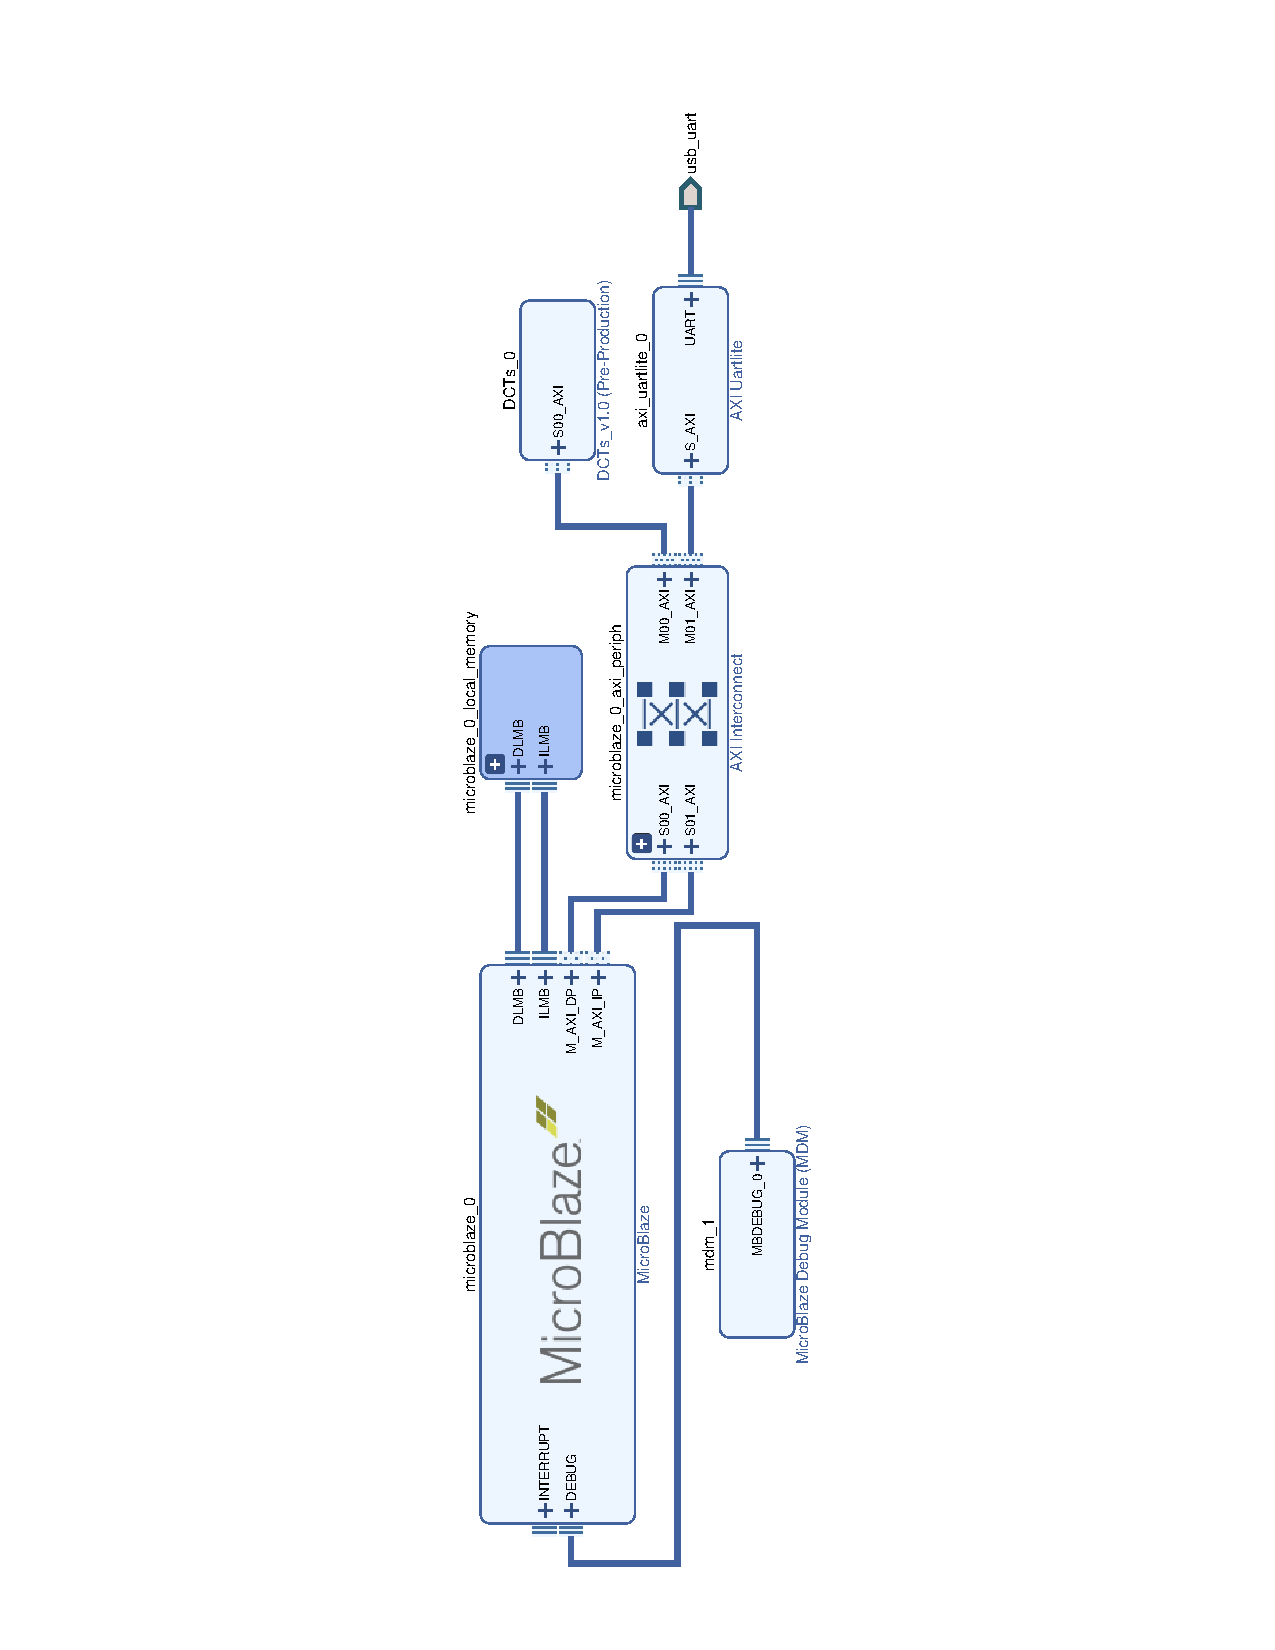
\includegraphics[width=\textwidth]{Figures/DCTCop.png}
              \caption{Diagrama de blocos implementado}
       \end{figure}       
\end{frame}

\note{
       \begin{itemize}[label=$\bullet$]
              \item Ultimo passo desta dissertação foi a integração da segunda arquitetura num design com Microblaze, num kit de hardware Nexys 4 da Digilent
              \item Micro-Processador ARM usado em ferramentas da Xilinx
              \item Prova de conceito para codificador completo
       \end{itemize}
}

\begin{frame}
       \frametitle{Implementação Nexys 4 - Resultados}
       \begin{equation*}
              f_{Max} = 101.9\,MHz
       \end{equation*}
       \begin{equation*}
              P = 50\,mW
       \end{equation*}
       \begin{table}[!htpb]
              \centering
              \caption{Frame rate máximo obtido na implementação com Nexys 4}
              \adjustbox{max height=\dimexpr\textheight-5.5cm\relax, max width=\textwidth}{
                     \begin{tabular}{ccccc} \toprule
                            \multirow{2}{*}{\textbf{Tamanho de Bloco}}   & \multicolumn{4}{c}{\textbf{Resolução}}                      \\
                                                               & $\mathbf{1280\times 720}$    & $\mathbf{1920\times 1080}$  & $\mathbf{3840\times 2160}$  & $\mathbf{7680\times 4320}$  \\ \toprule
                            $\mathbf{4\times 4}$                       & 37                      & 16                   & 4                    & 1  \\
                            $\mathbf{8\times 8}$                       & 44                      & 20                   & 5                    & 1  \\
                            $\mathbf{16\times 16}$                      & 63                      & 28                   & 7                    & 2  \\
                            $\mathbf{32\times 32}$                      & 98                      & 44                   & 11                   & 3  \\
                            $\mathbf{64\times 64}$                      & 161                     & 71                   & 18                   & 4  \\
                            \bottomrule
                     \end{tabular}    
              }
       \end{table}          
\end{frame}

\note{
       \begin{itemize}[label=$\bullet$]
              \item Vivado estima uma frequencia máxima de operação de aproximadamente 102 MHz
              \item 50 mW de potência consumida
              \item Frame rates baixos neste hardware, apesar do funcionamento ser o Esperado
              \item Justifica-se a necessidade de implementações em ASIC, capazes de frequencias de clock mais elevadas
       \end{itemize}
}

%%%%%%%%%%%%%%%%%%%%%%
% Conclusões e Trabalho Futuro
\section{Conclusões e Trabalho Futuro}

\note{
       \begin{itemize}[label=$\bullet$]
              \item
       \end{itemize}
}

\begin{frame}
       \frametitle{Conclusões}
       \begin{itemize}
              \item[\ding{51}] Estudo \emph{libaom} e identificação de características exploráveis
              \item[\ding{51}] Otimização do Software de referência
              \begin{itemize}[label=$\bullet$]
                     \item Redução em 81\% da memória utilizada nas aproximações do cosseno
                     \item Prova da possibilidade de usar 8 bits sem impacto na qualidade da codificação
              \end{itemize} 
              \item[\ding{51}] Construção de arquiteturas em hardware para o kernel da DCT
              \begin{itemize}[label=$\bullet$]
                     \item Duas implementações distintas
              \end{itemize} 
              \item[\ding{51}] Implementação em Nexys 4
              \begin{itemize}[label=$\bullet$]
                     \item Prova de conceito em Codificador Completo
              \end{itemize} 
       \end{itemize}
\end{frame}

\note{
       \begin{itemize}[label=$\bullet$]
              \item Objetivos atingidos
              \item Otimização do software de referência com estudo das características de codificação do AV1
              \item Contrução de arquiteturas de hardware funcionais para a DCT, e implementação prática da segunda
       \end{itemize}
}
\begin{frame}
       \frametitle{Trabalho Futuro}
       \begin{itemize}[label=$\bullet$]
              \item[\ding{212}] Integração dos restantes kernels
              \item[\ding{212}] Teste com \emph{libaom} em FPGA
              \item[\ding{212}] Síntese para ASIC
       \end{itemize}
\end{frame}

\note{
       \begin{itemize}[label=$\bullet$]
              \item Integração dos restantes kernels 
              \item Teste da arquitetura de hardware com libaom em FPGA com interface com muita largura de banda (PCIE por exemplo)
              \item Sintese para ASIC para obter frequencia máxima de operação
       \end{itemize}
}

\begin{frame}[standout, c]
       \begin{center}
              \Huge \textbf{Obrigado!}\\
       \end{center}
\end{frame}

\note{
       \begin{itemize}[label=$\bullet$]
              \item 
       \end{itemize}
}

\begin{frame}[standout,c]
       \begin{center}
              \Huge \textbf{Discussão}\\ \vspace{1cm}
              \Large Co-processador da Transformada para o Codificador de Vídeo AV1 \\ \vspace{.5cm}
              \large Miguel Oliveira Inocêncio      \\ \vspace{1.5cm}
              \begin{columns}
                     \column{0.3\textwidth}
                            \centering
                            \large Professor\\
                            \large Armando Pinho\\
                            \small \textbf{Presidente do Júri}
                     \column{0.3\textwidth}
                            \centering
                            \large Professor\\
                            \large Pedro Assunção\\
                            \small \textbf{Arguente Principal}
                     \column{0.3\textwidth}
                            \centering
                            \large Professor\\
                            \large António Navarro\\
                            \small \textbf{Orientador}
              \end{columns}
       \end{center}
\end{frame}

\note{
       \begin{itemize}[label=$\bullet$]
              \item 
       \end{itemize}
}

\end{document}